\documentclass[11pt]{article}

\hoffset        2mm 
\voffset        -15mm
\oddsidemargin  0mm
\topmargin      0.30in
\textwidth      6.25in
\textheight     9in

\usepackage[parfill]{parskip}
\usepackage{graphicx}
\usepackage{amsmath}
%\usepackage{mathtools}
\usepackage{booktabs}
\usepackage{enumerate}
\usepackage{listings}
\usepackage{float}
\usepackage{bigints}
\usepackage{caption}
\usepackage{subcaption}
\usepackage{afterpage}
\usepackage{epstopdf}
\usepackage{commath}
\usepackage{amssymb}
\usepackage{titlesec}

% Section parameters
\setcounter{secnumdepth}{4}
\titleformat{\paragraph}
{\normalfont\normalsize\bfseries}{\theparagraph}{1em}{}
\titlespacing*{\paragraph}
{0pt}{3.25ex plus 1ex minus .2ex}{1.5ex plus .2ex}

\begin{document}


\begin{center}
{\Large Higher-Order DGFEM Transport Calculations on Polytope Meshes for Massively-Parallel Architectures}\\[8mm]
{Michael W. Hackemack} \\[2mm]
{\em \small Department of Nuclear Engineering, Texas A\&M University, College Station, TX 77843, USA} \\[1mm]
{\em mike\_hack@tamu.edu} \\[6mm]
\end{center}

%%%%%%%%%%%%%%%%%%%%%%%%%%%%%%%%%%%%%%%%%%%%%%%%%%%%%%%%%%%%%%%%%%%%%%
%%%%%%%%%%%%%%%%%%%%%%%%%%%%%%%%%%%%%%%%%%%%%%%%%%%%%%%%%%%%%%%%%%%%%%
\section{Introduction}
\label{sec::intro}

The discontinuous Galerkin finite element method (DGFEM) has been widely used to solve the radiation transport equation using the discrete ordinates ($S_N$) approximation \cite{reed1973triplet}. The standard, multigroup $S_N$ neutral particle transport equation (without the position parameter) for a given direction, $\vec{\Omega}_m$, and energy group, $g$, is given by the following,

\begin{equation}
\label{eq::trans_eq}
\vec{\Omega}_m \cdot \vec{\nabla} \Psi_{m,g} + \sigma_{t,g} \Psi_{m,g} (\vec{\Omega}_m) = \sum_{g'=1}^G \sum_{n=0}^{N_a} \frac{2n+1}{4 \pi} \sum_{k=-n}^{n} \left[ \sigma_{s,n}^{g' \rightarrow g}  \Phi_{n,k,g'} Y_{n,k} (\vec{\Omega}_m) + Q_{n,k,g}  \right] ,
\end{equation}

\noindent where $\sigma_{t,g}$ is the total macroscopic cross section, $\sigma_{s,n}^{g' \rightarrow g}$ are the macroscopic scattering moments, $\Phi_{n,k,g'}$ are the solution spherical harmonic moments, and $Q_{n,k,g}$ are the distributed source moments \cite{lewis1984computational}. 

We next restrict our problem to a single energy group and simplify the right-hand-side sources, lay down a mesh, $\mathbb{T}_h$, over our problem, multiply by a basis function, $b_m$, analyze a single cell, $K$, integrate over the volume of the cell, and apply Gauss' theorem to yield,

\begin{equation}
\label{eq::disc_trans_eq_cellK}
- \left( \vec{\Omega}_m \cdot  \vec{\nabla} b_m, \Psi_{m} \right)_{K} + \sum_{f=1}^{N_f^K} \Big< ( \vec{\Omega}_m \cdot \vec{n}_f ) \, b_m, \tilde{\Psi}_m  \Big>_{f}  + \Big(  \sigma_{t} b_m ,   \Psi_{m} \Big)_{K} = \left(  b_m ,   Q_m \right)_{K}
\end{equation}

\noindent where $\vec{n}_f$ is the outward normal direction for face $f$ on the cell $K$ boundary and $N_f^K$ is the number of faces on cell $K$. The volume and surface inner products have the form,

\begin{equation}
\label{eq::inner_prod}
\Big( u,v \Big)_K \equiv \int_K u \, v \, d \vec{r} \qquad \text{and} \qquad \Big< u,v \Big>_f \equiv \int_f u \, v \, d s ,
\end{equation}

\noindent respectively. The across-cell boundary flux, $\tilde{\Psi}_m$, is boundary dependent. We apply the ubiquitous {\em upwind scheme} 

\begin{equation}
\label{eq::upwind_eqs}
\tilde{\Psi}_m (\vec{r})  = 
\begin{cases}
\Psi_m^{-} , & \partial K^+ \\
\Psi_m^{+}, & \partial K^- \backslash \partial \mathcal{D} \\
\Psi_m^{inc}, & \partial K^- \cap \partial \mathcal{D}^d \\
\Psi_{m'}^{-}, & \partial K^- \cap \partial \mathcal{D}^r
\end{cases}
\end{equation}

\noindent where the trace is defined as: $\Psi_m^{\pm} (\vec{r}) \equiv \lim_{s \rightarrow 0^{\pm}} \Psi_m \Big( \vec{r} + s (\vec{\Omega}_m \cdot \vec{n}) \vec{n} \Big)$. We then insert the upwind notation of Eq. (\ref{eq::upwind_eqs}) into Eq. (\ref{eq::disc_trans_eq_cellK}) to yield the full set of spatially discretized equations for cell $K$,

\begin{equation}
\label{eq::full_cellK_disc}
\begin{aligned}
-  \Big( \vec{\Omega}_m \cdot  & \vec{\nabla} b_m, \Psi_{m} \Big)_{K}   + \Big(  \sigma_{t} b_m ,   \Psi_{m} \Big)_{K} +  \Big< ( \vec{\Omega}_m \cdot \vec{n} ) \, b_m, {\Psi}_m^{-}  \Big>_{\partial K^+}  \\
  + & \Big< ( \vec{\Omega}_m \cdot \vec{n} ) \, b_m, {\Psi}_m^{+}  \Big>_{\partial K^- \backslash \partial \mathcal{D}}  + \Big< ( \vec{\Omega}_m \cdot \vec{n} ) \, b_m, {\Psi}^{-}_{m'}  \Big>_{\partial K^- \cap \partial \mathcal{D}^r}  \\
= & \left(  b_m ,   Q_m \right)_{K} - \Big< ( \vec{\Omega}_m \cdot \vec{n} ) \, b_m, {\Psi}_m^{inc}  \Big>_{\partial K^- \cap \partial \mathcal{D}^d} 
\end{aligned} \, .
\end{equation}

At this point we note that we have not specified a mesh or basis function type. We have simply left them as an unspecified dual. In base finite element theory, the basis functions are collections of polynomial functions with measure on local elements within the domain \cite{ern2013theory}. A particular application of the Bramble-Hilbert lemma states that we can achieve error convergence rates between the true solution,$u$, and the discretized solution, $u_h$, by,

\begin{equation}
\label{eq::bf_conv_rate_h}
|| u - u_h ||_{L_2} = C h^{p+1}
\end{equation}

\noindent where $h$ is the maximum diameter of a mesh element, $p$ is the polynomial order of the basis functions, and $C$ is a constant independent of the mesh \cite{bramble1970estimation}. If $h$ is difficult to estimate for a particular mesh type, we can proportionally relate it to the number of spatial degrees of freedom in the problem: $N_{dof} \propto h^{-d}$, where $d$ is the dimensionality of the problem (1,2,3). Using this relation, Eq. (\ref{eq::bf_conv_rate_h}) can be rewritten to be dependent on the number of spatial degrees of freedom,

\begin{equation}
\label{eq::bf_conv_rate_DOF}
|| u - u_h ||_{L_2} = C N_{dof}^{- \frac{p+1}{d}},
\end{equation}

\noindent where we note that the constants, $C$, in Eqs. (\ref{eq::bf_conv_rate_h}) and (\ref{eq::bf_conv_rate_DOF}) are not the same. We plot the relations of Eqs. (\ref{eq::bf_conv_rate_h}) and (\ref{eq::bf_conv_rate_DOF}) in Figure \ref{fig::conv_rates} for different polynomial orders. We can see from the relationship of mesh cell size and number of spatial degrees of freedom to the error, that using basis functions with higher-order polynomial interpolations leads to improved convergence rates. As long as the number of spatial degrees of freedom does not grow proportionally to the polynomial order, we expect to achieve more accurate solution estimates in relation to the work required to solve the problem with higher-order interpolants.

\begin{figure}[hbt]
\centering
	\begin{subfigure}[b]{0.475\textwidth}
		\centering
		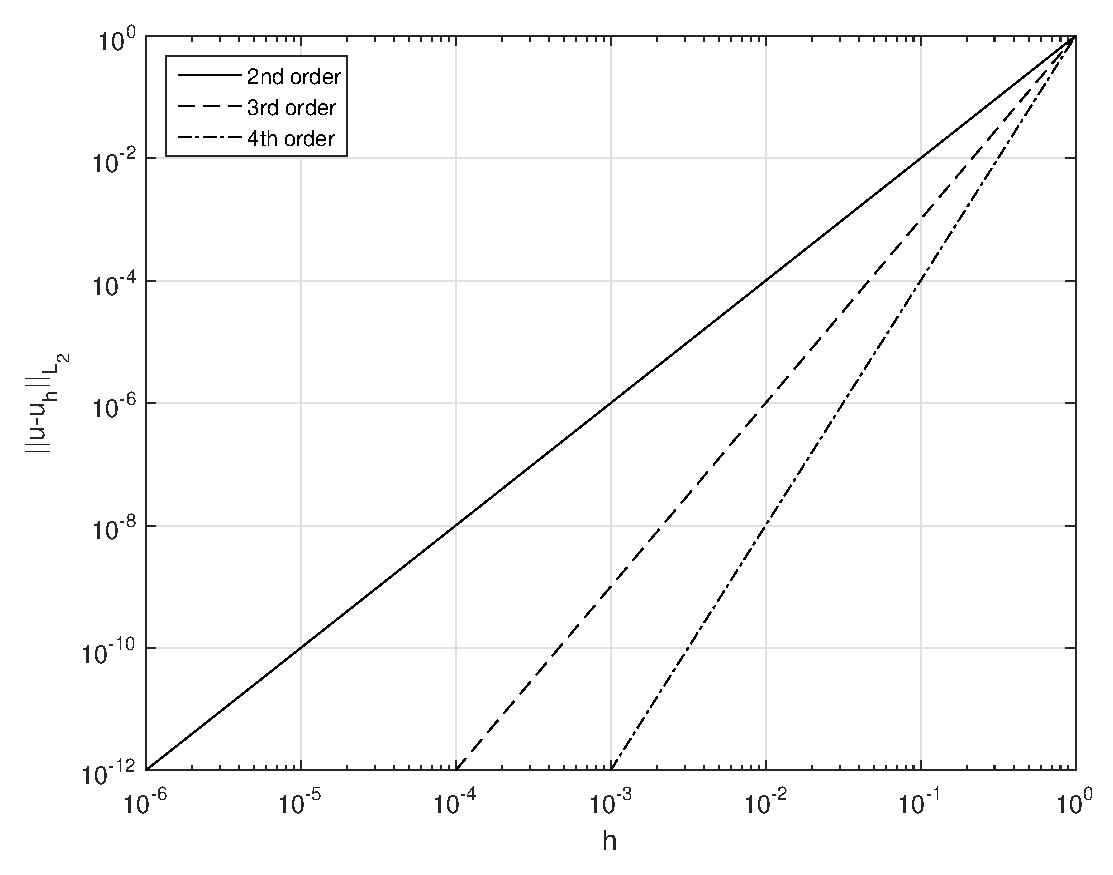
\includegraphics[width=\textwidth]{figures/hconv_larger.eps}
		\caption{}
	\end{subfigure}
	\hfill
	\begin{subfigure}[b]{0.475\textwidth}
		\centering
		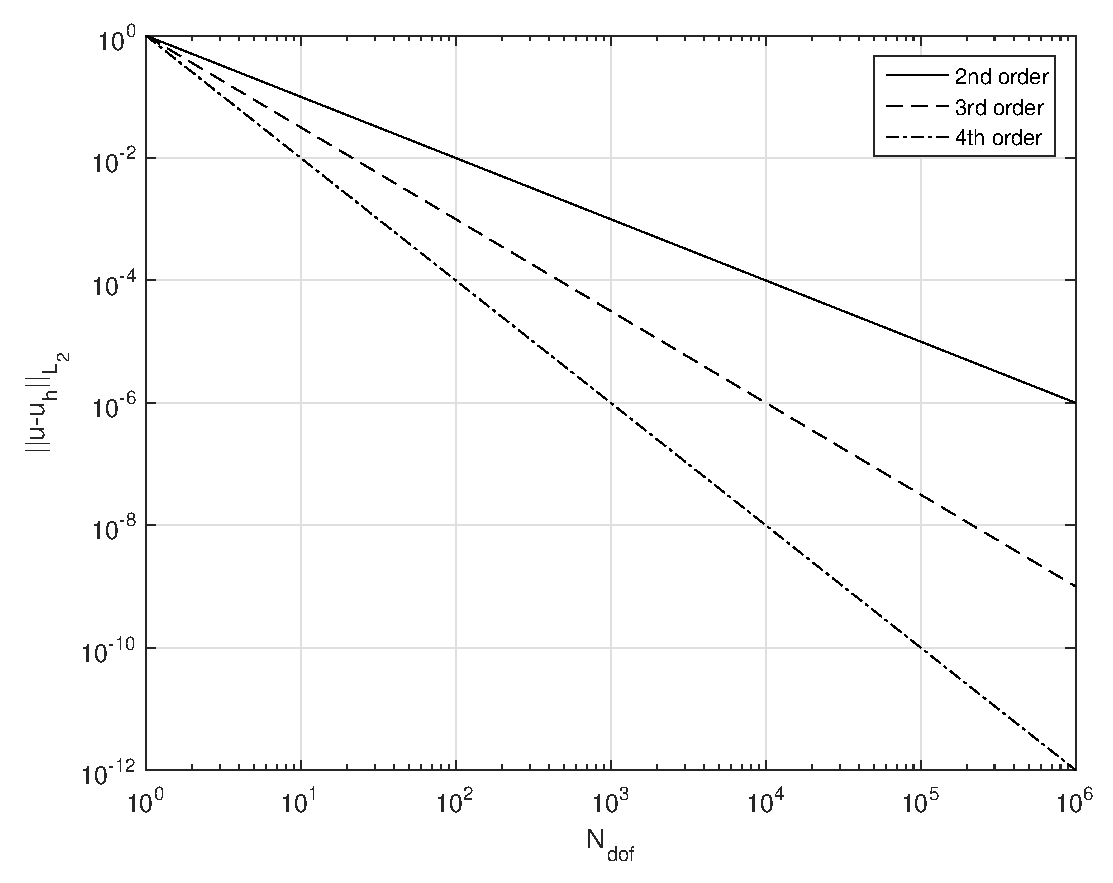
\includegraphics[width=\textwidth]{figures/Nconv_larger.eps}
		\caption{}
	\end{subfigure}
\caption{Theoretical convergence rates of transport solutions with no irregularity based on (a) mesh cell measure and (b) number of spatial degrees of freedom.}
\label{fig::conv_rates}
\end{figure}

For the finite element method, analysis has typically been performed on simple element types: triangles and quadrilaterals in 2D and tetrahedra and hexahedra in 3D \cite{akin1982application}. However, in more recent years there has been a growing interest in different research communities to apply the finite element method to polytope mehes (polygons and polyhedra). Some of the main benefits for using arbitrary polygonal/polyhedral meshes are the following:

\vspace{4mm}
\begin{enumerate}
	\item Polytope mesh cells are now being employed in other physics communities - most notably computational fluid dynamics (CFD)\cite{ref::star_CCM};
	\item They are believed to reduce the number of unknowns to solve with equivalent accuracy;
	\item They can reduce cell/face counts which can reduce algorithm wallclock times depending on the solution method;
	\item They can allow for transition elements between different portions of the domain (e.g., tetrahedral elements bordering hexahedral elements at the border of the boundary layer);
	\item They can easily be split along cut planes - allowing the mesh to be partitioned into regular or irregular divisions as well as be generated by simplical meshing techniques across processor sets in parallel;
	\item Hanging nodes from non-conforming meshes, like those that naturally arise from locally refined/adapted meshes, are no longer necessary. 
\end{enumerate}
\vspace{4mm}

It is because of both these benefits (higher-order FEM basis functions and polytope meshes) which have governed the work going into this dissertation. We seek to analyze and compare different linear polygonal basis functions  for use in DGFEM transport calculations. We then continue this analysis with a quadratic serendipity extension to these linear polygonal basis functions \cite{rand2014quadratic}. We then wish to take the knowledge gained from this polytope DGFEM transport calculation analysis to drive further research into the preconditioning of the DGFEM transport equation for use in massively-parallel computer architectures.

The rest of this proposal is organized as follows. In Section \ref{sec::PS}, we give a brief overview of the existing methodologies used for DGFEM transport. In Section \ref{sec::CW}, we present an overview of the work that has been completed to date. In Section \ref{sec::OW}, we present the remaining work that still needs to be accomplished. Finally, Section \ref{sec::ER} provides a summary of all the expected results that is to be completed with this dissertation work.

%%%%%%%%%%%%%%%%%%%%%%%%%%%%%%%%%%%%%%%%%%%%%%%%%%%%%%%%%%%%%%%%%%%%%%
%%%%%%%%%%%%%%%%%%%%%%%%%%%%%%%%%%%%%%%%%%%%%%%%%%%%%%%%%%%%%%%%%%%%%%
\section{Existing Methodology}
\label{sec::PS}
% Transport and FEM Portion

% DSA Portion
The ability to efficiently invert the transport (streaming and collision) operator does not necessarily mean that transport solutions can be easily obtained. In general, radiation transport solutions are obtained iteratively. The simplest and widely-used method is a fixed-point scheme ({\em i.e.} richardson iteration) ubiquitously called source iteration (SI) in the transport community. Unfortunately, the iteration process of SI can converge arbitrarily slowly if the problem is optically thick \cite{ref::adams_larsen_iter_methods}. This corresponds to long mean free paths for neutronics problems. This also corresponds to time steps and material heat capacities tending to infinity and zero, respectively, for thermal radiative transport (TRT) problems.

For these problem regimes in which solution is prohibitively slow, additional steps should be taken to speed up, or accelerate, solution convergence \cite{ref::adams_larsen_iter_methods}. The most used methods to assist in solution convergence are often called synthetic acceleration techniques. These techniques were first introduced by Kopp  \cite{kopp1963synthetic} and Lebedev \cite{lebedevI} in the 1960's. From Kopp's and Lebedev's work, Gelbard and Hageman then introduced two synthetic acceleration options for the low-order operator: diffusion and $S_2$ \cite{gelbard1969synthetic}. Their diffusion preconditioning led to efficient convergence properties on fine spatial meshes. Reed then showed that Gelbard and Hageman's diffusion preconditioning would yield a diverging system for coarse meshes \cite{reed1971effectiveness}. At this point in time, no one knew if an unconditionally efficient acceleration method could be derived.

Then in 1976, Alcouffe proposed a remedy to Gelbard and Reed that he called diffusion synthetic acceleration (DSA) \cite{alcouffe1976stable,alcouffe1977DSA,alcouffe1977diffusion}. He showed that if you derived the diffusion operator consistently with the discretized transport operator, then SI could be accelerated with DSA in an efficient and robust manner. Larsen and McCoy then demonstrated that unconditional stability required that consistency be maintained in both spatial and angular discretization in their four-step procedure \cite{larsen1982unconditionally_I,larsen1982unconditionally_II}. However, Adams and Martin then showed that partially-consistent diffusion discretizations could effectively accelerate DFEM discretizations of the neutron transport equation \cite{ref::dsa_DFEM_adams_martin}. Their modified-four-step procedure (M4S), based on Larsen and McCoy's work, was shown to be unconditionally stable for regular geometries, but divergent for unstructured multi-dimensional meshes \cite{warsa2002fully}. In more recent years, alternate discretizations for the diffusion operator have been applied to unstructured multi-dimensional grids. These include the partially consistent Wareing-Larsen-Adams (WLA) DSA \cite{ref::WLA_DSA}, the fully consistent DSA (FCDSA) \cite{warsa2002fully}, and the partially consistent MIP DSA \cite{ref::DSA_wang_ragusa,wang2009adaptive,turcksin2014discontinuous}.

Most recently, the partially consistent MIP DSA method has been shown to be an unconditionally stable acceleration method for the 2D DFEM transport equation on unstructured meshes. Wang showed that it acted as an effective preconditioner for higher-order DFEM discretizations on triangles \cite{ref::DSA_wang_ragusa,wang2009adaptive}. Turcksin and Ragusa then extended the work to arbitrary polygonal meshes \cite{turcksin2014discontinuous}. The MIP diffusion operator is symmetric positive definite (SPD) and was shown to be efficiently invertible with preconditioned conjugate gradient (PCG) and advanced preconditioners such as algebraic multi-grid (AMG) \cite{turcksin2014discontinuous}.

%%%%%%%%%%%%%%%%%%%%%%%%%%%%%%%%%%%%%%%%%%%%%%%%%%%%%%%%%%%%%%%%%%%%%%
%%%%%%%%%%%%%%%%%%%%%%%%%%%%%%%%%%%%%%%%%%%%%%%%%%%%%%%%%%%%%%%%%%%%%%
\section{Current Work}
\label{sec::CW}

We have just defined the current state of the art for DGFEM transport calculations on arbitrary meshes for massively-parallel problems. We also presented appropriate DSA preconditioners. Next, we define the work to be performed for this dissertation as well as some preliminary results. Section \ref{sec::CW_poly} details higher-order transport calculations on 2D polygons. Section \ref{sec::CW_DSA} details extending MIP DSA preconditioning for 3D massively parallel problems including accelerating problems dominated by thermal neutron upscattering.

%%%%%%%%%%%%%%%%%%%%%%%%%%%%%%%%%%%%%%%%%%%%%%%%%%%%%%%%%%%%%%%%%%%%%%
\subsection{DGFEM Transport Calculations on Polygonal Meshes}
\label{sec::CW_poly}

The first topical area of research that this dissertation work will focus on is the use of higher-order polygonal basis functions to solve the DGFEM $S_N$ transport equation. 

\begin{figure}
\label{fig::2D_Linear_Summary_unit_square_basis_functions}
\centering
	\begin{subfigure}[b]{0.225\textwidth}
		\centering
		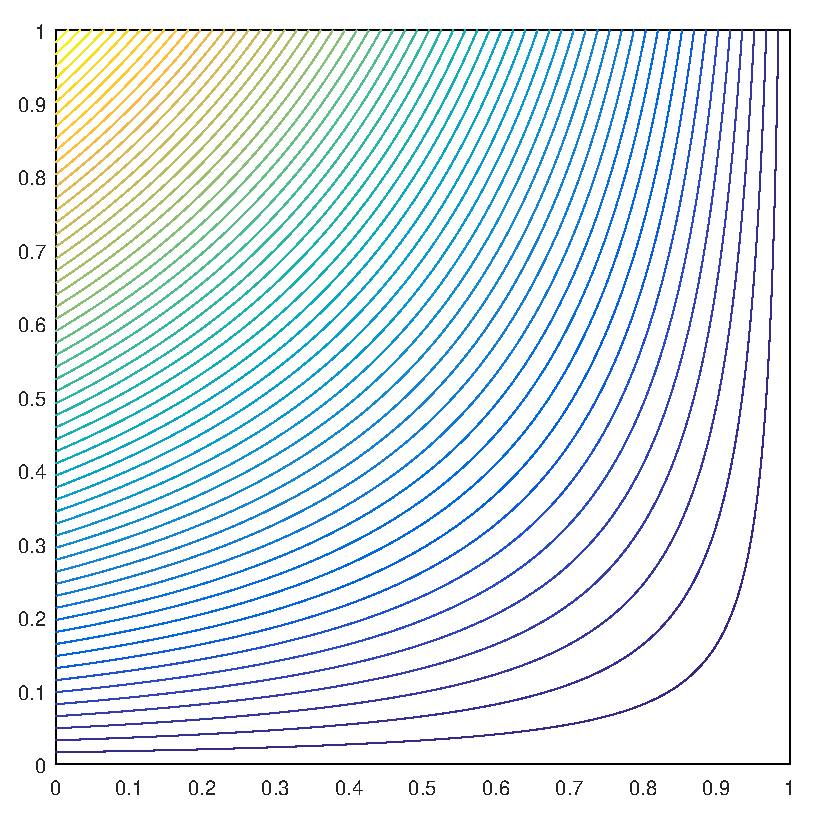
\includegraphics[width=\textwidth]{figures/square_WACHSPRESS1_contour_b4.eps}
		\caption{}
	\end{subfigure}
	\hspace{1cm}
	\begin{subfigure}[b]{0.225\textwidth}
		\centering
		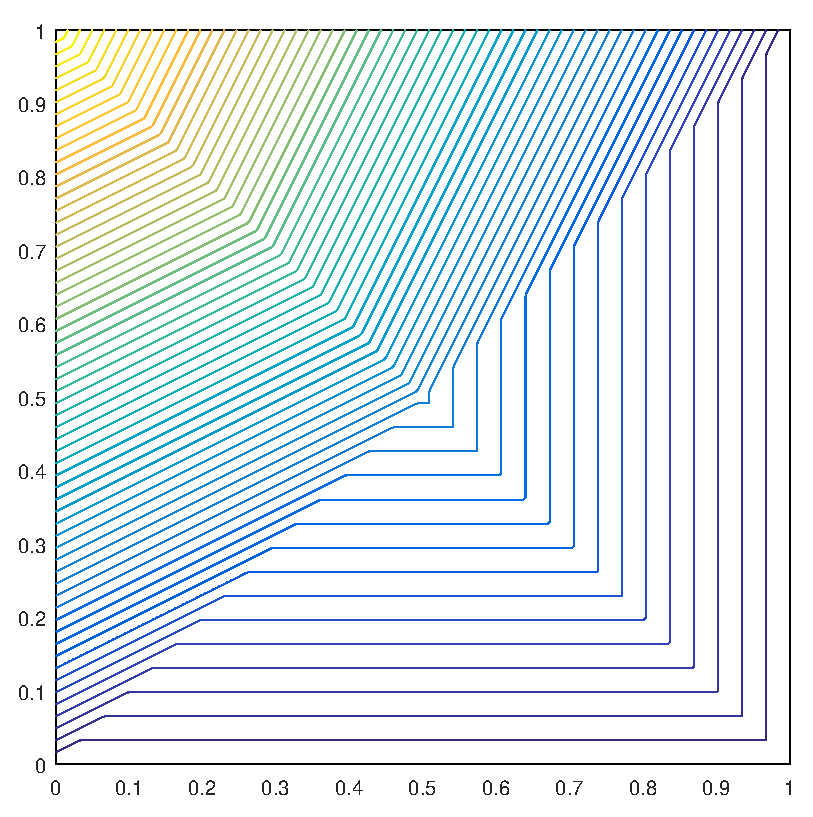
\includegraphics[width=\textwidth]{figures/square_PWLD1_contour_b4.eps}
		\caption{}
	\end{subfigure}
	\vfill
	\begin{subfigure}[b]{0.225\textwidth}
		\centering
		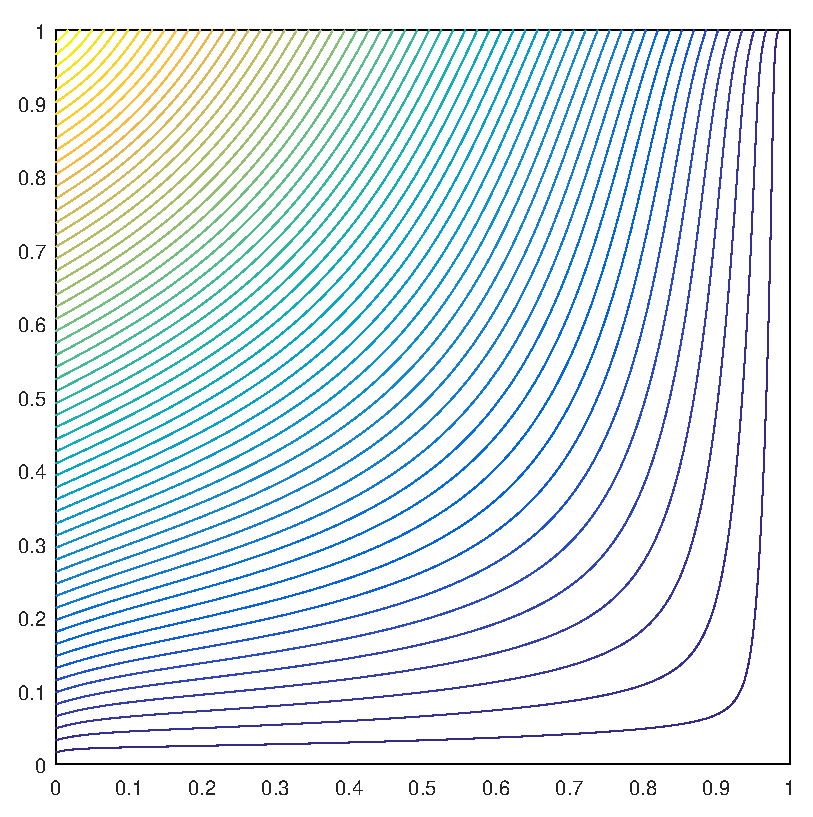
\includegraphics[width=\textwidth]{figures/square_MV1_contour_b4.eps}
		\caption{}
	\end{subfigure}
	\hspace{1cm}
	\begin{subfigure}[b]{0.225\textwidth}
		\centering
		\includegraphics[width=\textwidth]{figures/square_MAXENT1_contour_b4.eps}
		\caption{}
	\end{subfigure}
\caption{Contour plots of the different linear basis functions on the unit square located at vertex (0,1): (a) Wachspress, (b) PWL, (c) mean value, and (d) maximum entropy.}
\end{figure}



The functional interpolation requirements for the linear basis functions are

\begin{equation}
\label{eq::poly_completeness}
\begin{aligned}
\sum_{i=1}^{N_K} \,&b_i(\vec{x}) = 1 \\
\sum_{i=1}^{N_K}\, & b_i(\vec{x})  \vec{x}_i  =\vec{x}
\end{aligned}
\end{equation}

\noindent 

\begin{table}[hbt]
\label{tab::lin_poly_summary}
\caption{Summary of the properties of the linear polygonal basis functions used in this work.}
\centering
\begin{tabular}{|c|c|c|c|c|}
\hline
Basis Function & Dimension & Polytope Types & Integration & Direct/Iterative \\
\hline \hline
Wachspress	&2D/3D&	Convex&	Numerical	&Direct\\ \hline
PWL&	1D/2D/3D&	Convex/Concave&	Analytical	&Direct\\ \hline
Mean Value&	2D&	Convex/Concave&	Numerical	&Direct\\ \hline
Max Entropy&	1D/2D/3D	&Convex/Concave&	Numerical&	Iterative\\ \hline
\end{tabular}
\end{table}

\begin{figure}[hbt]
\centering
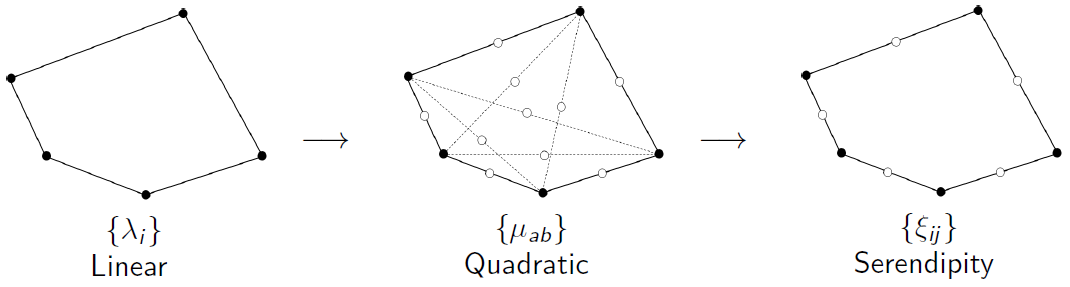
\includegraphics[width=\textwidth]{figures/linear_to_quad_process.png}
\caption{Overview of the process to construct the quadratic serendipity basis functions on polygons. The filled dots correspond to basis functions that maintain the Lagrange property while empty dots do not.}
\label{fig::lin_to_quad_process}
\end{figure}

\begin{figure}
\label{fig::2D_Quadratic_Summary_unit_square_basis_functions_b4}
\centering
	\begin{subfigure}[b]{0.25\textwidth}
		\centering
		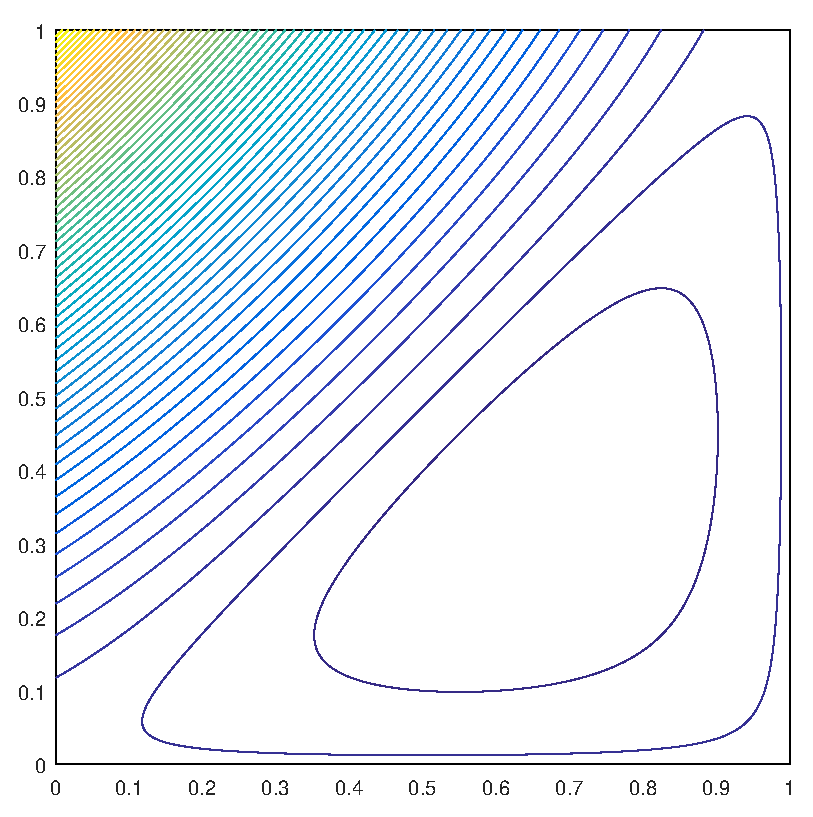
\includegraphics[width=\textwidth]{figures/square_WACHSPRESS2_contour_b4.eps}
		\caption{}
	\end{subfigure}
	\hspace{1cm}
	\begin{subfigure}[b]{0.25\textwidth}
		\centering
		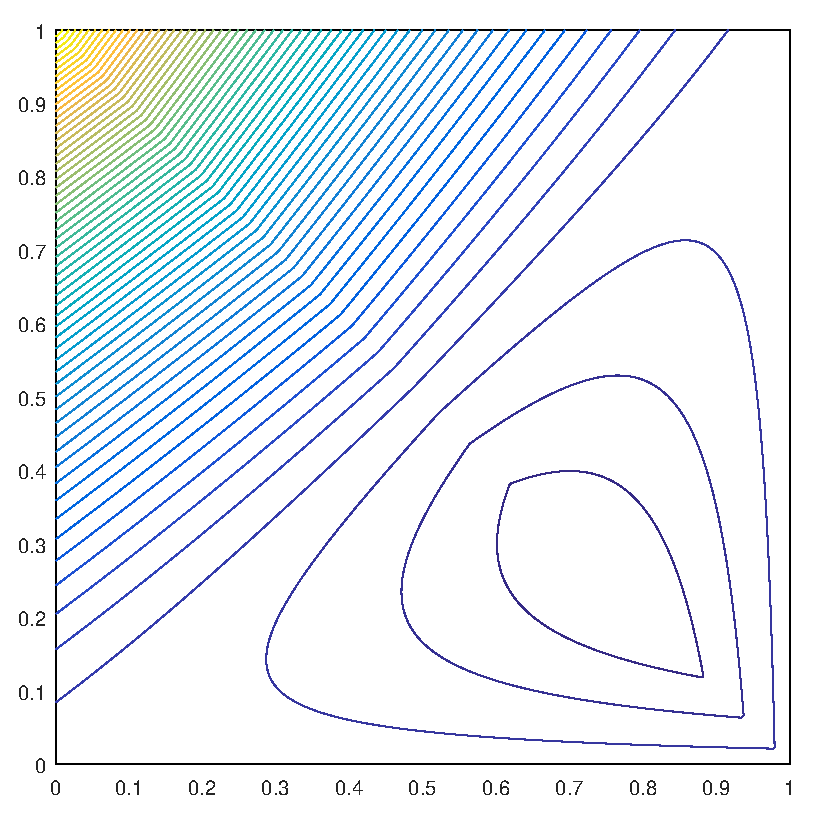
\includegraphics[width=\textwidth]{figures/square_PWLD2_contour_b4.eps}
		\caption{}
	\end{subfigure}
	\vfill
	\begin{subfigure}[b]{0.25\textwidth}
		\centering
		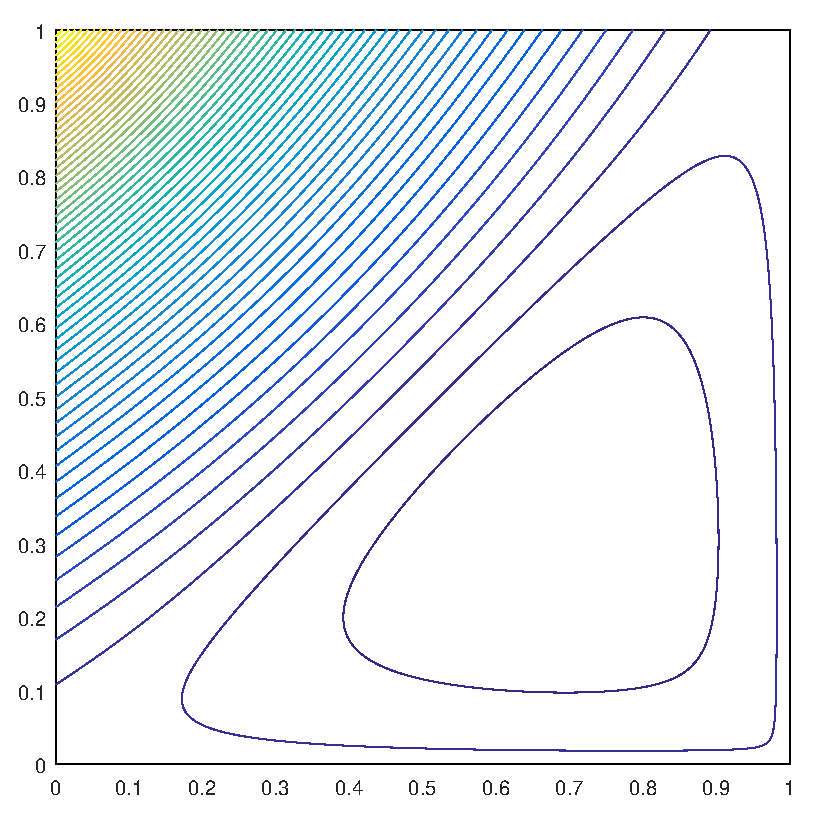
\includegraphics[width=\textwidth]{figures/square_MV2_contour_b4.eps}
		\caption{}
	\end{subfigure}
	\hspace{1cm}
	\begin{subfigure}[b]{0.25\textwidth}
		\centering
		\includegraphics[width=\textwidth]{figures/square_MAXENT2_contour_b4.eps}
		\caption{}
	\end{subfigure}
\caption{Contour plots of the different quadratic serendipity basis functions on the unit square located at vertex (0,1): (a) Wachspress, (b) PWL, (c) mean value, and (d) maximum entropy.}
\end{figure}

\begin{figure}
\label{fig::2D_Quadratic_Summary_unit_square_basis_functions_b8}
\centering
	\begin{subfigure}[b]{0.25\textwidth}
		\centering
		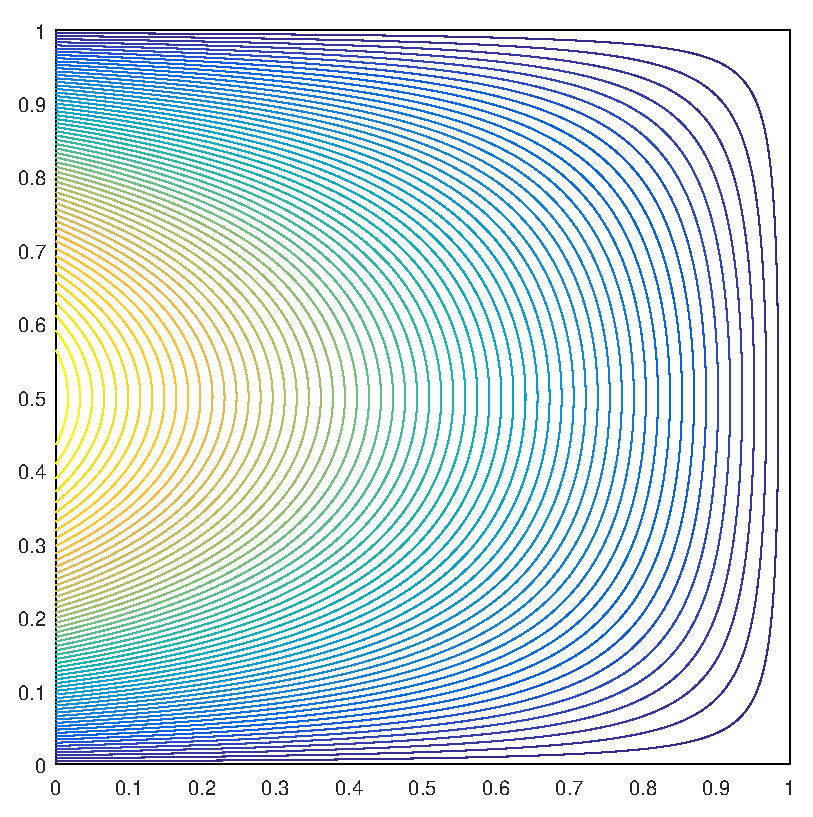
\includegraphics[width=\textwidth]{figures/square_WACHSPRESS2_contour_b8.eps}
		\caption{}
	\end{subfigure}
	\hspace{1cm}
	\begin{subfigure}[b]{0.25\textwidth}
		\centering
		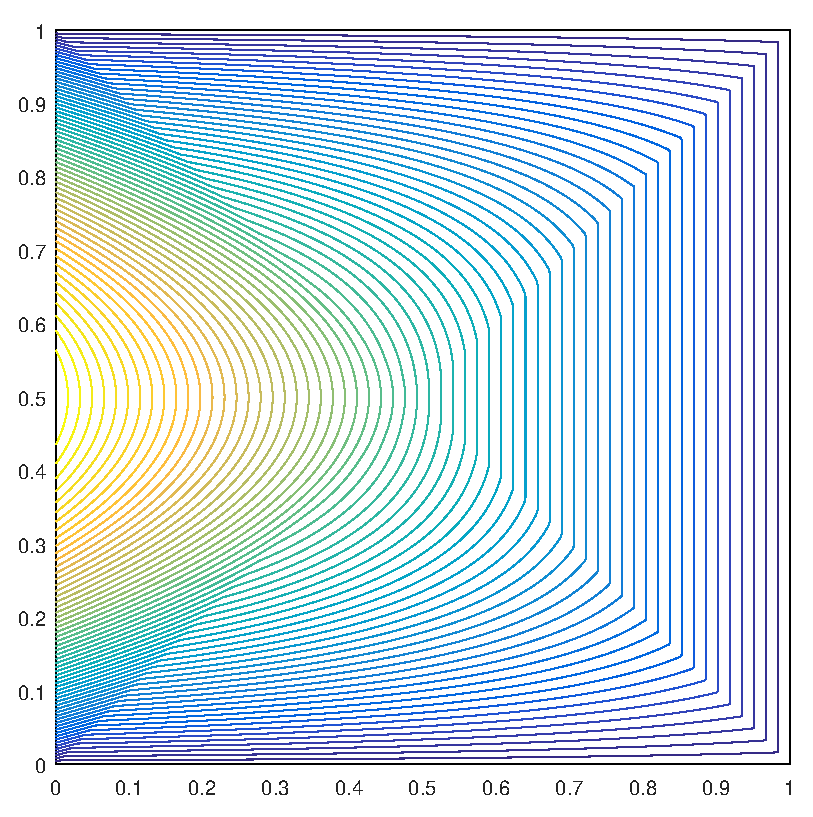
\includegraphics[width=\textwidth]{figures/square_PWLD2_contour_b8.eps}
		\caption{}
	\end{subfigure}
	\vfill
	\begin{subfigure}[b]{0.25\textwidth}
		\centering
		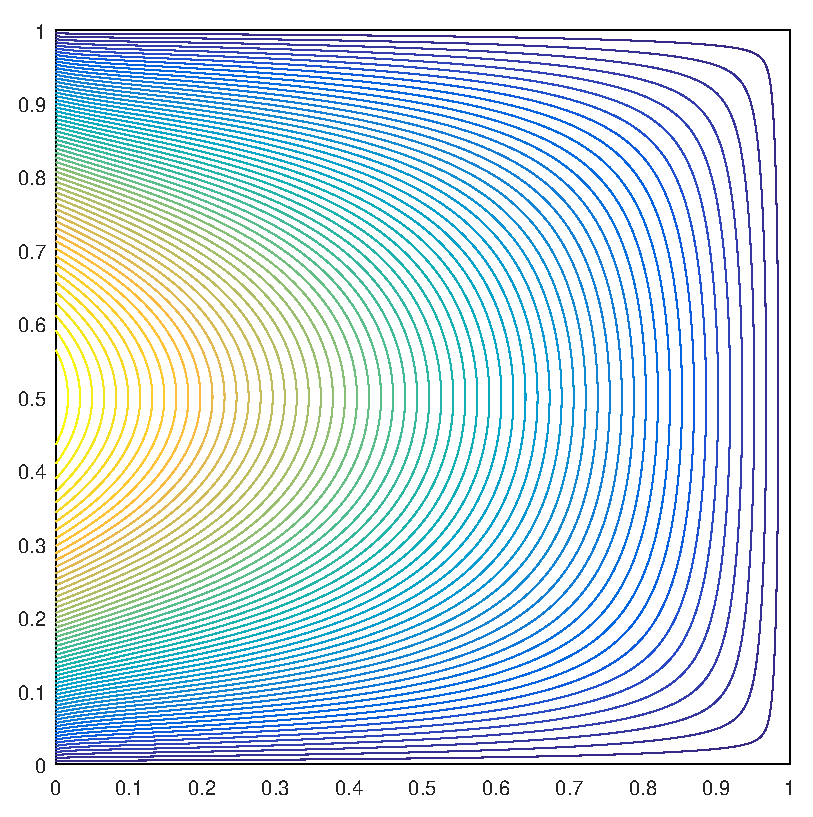
\includegraphics[width=\textwidth]{figures/square_MV2_contour_b8.eps}
		\caption{}
	\end{subfigure}
	\hspace{1cm}
	\begin{subfigure}[b]{0.25\textwidth}
		\centering
		\includegraphics[width=\textwidth]{figures/square_MAXENT2_contour_b8.eps}
		\caption{}
	\end{subfigure}
\caption{Contour plots of the different quadratic serendipity basis functions on the unit square located at vertex (0,1/2): (a) Wachspress, (b) PWL, (c) mean value, and (d) maximum entropy.}
\end{figure}

Having identified the 2D linear polygonal finite element basis functions of interest along with the means to convert them to the quadratic serendipity space, we now wish to analyze their numerical characteristics. First, we wish to verify that all the basis functions can capture an exactly-linear solution on polygonal meshes. We do this by considering the simplified 1-group transport equation,

\begin{equation}
\label{eq::lin_trans_eq}
\mu \frac{\partial  \psi}{\partial x} + \eta \frac{\partial  \psi}{\partial y} + \sigma_t \psi = Q(x,y,\mu,\eta),
\end{equation}

\noindent with the following angular and scalar flux solutions,

\begin{equation}
\label{eq::BF_Results_Linear_fluxsols}
\begin{aligned}
\Psi (x,y,\mu,\eta) &= ax + by + c \mu + d\eta + e,\\
\Phi (x,y) &= 2 \pi \left( ax + by  + e \right).
\end{aligned} 
\end{equation}

\noindent Inserting the angular flux solution of Eq. (\ref{eq::BF_Results_Linear_fluxsols}) into Eq. (\ref{eq::lin_trans_eq}), gives the appropriate functional form for the right-hand-source that yields an exactly-linear solution. Using the level-symmetric quadrature set then guaranties that the linearly-dependent angular terms of the angular flux integrate to 0. We have analyzed all the polygonal basis functions on several different meshes. Figure \ref{fig::lin_sol} presents how the PWL basis functions capture an exactly-linear transport solution on two meshes: a polygonal mesh and a highly-distorted quadrilateral mesh. All the basis functions capture this behavior but we do not present these results for brevity.

\vspace{2mm}
\begin{figure}[hbt]
\centering
	\begin{subfigure}[b]{0.42\textwidth}
		\centering
		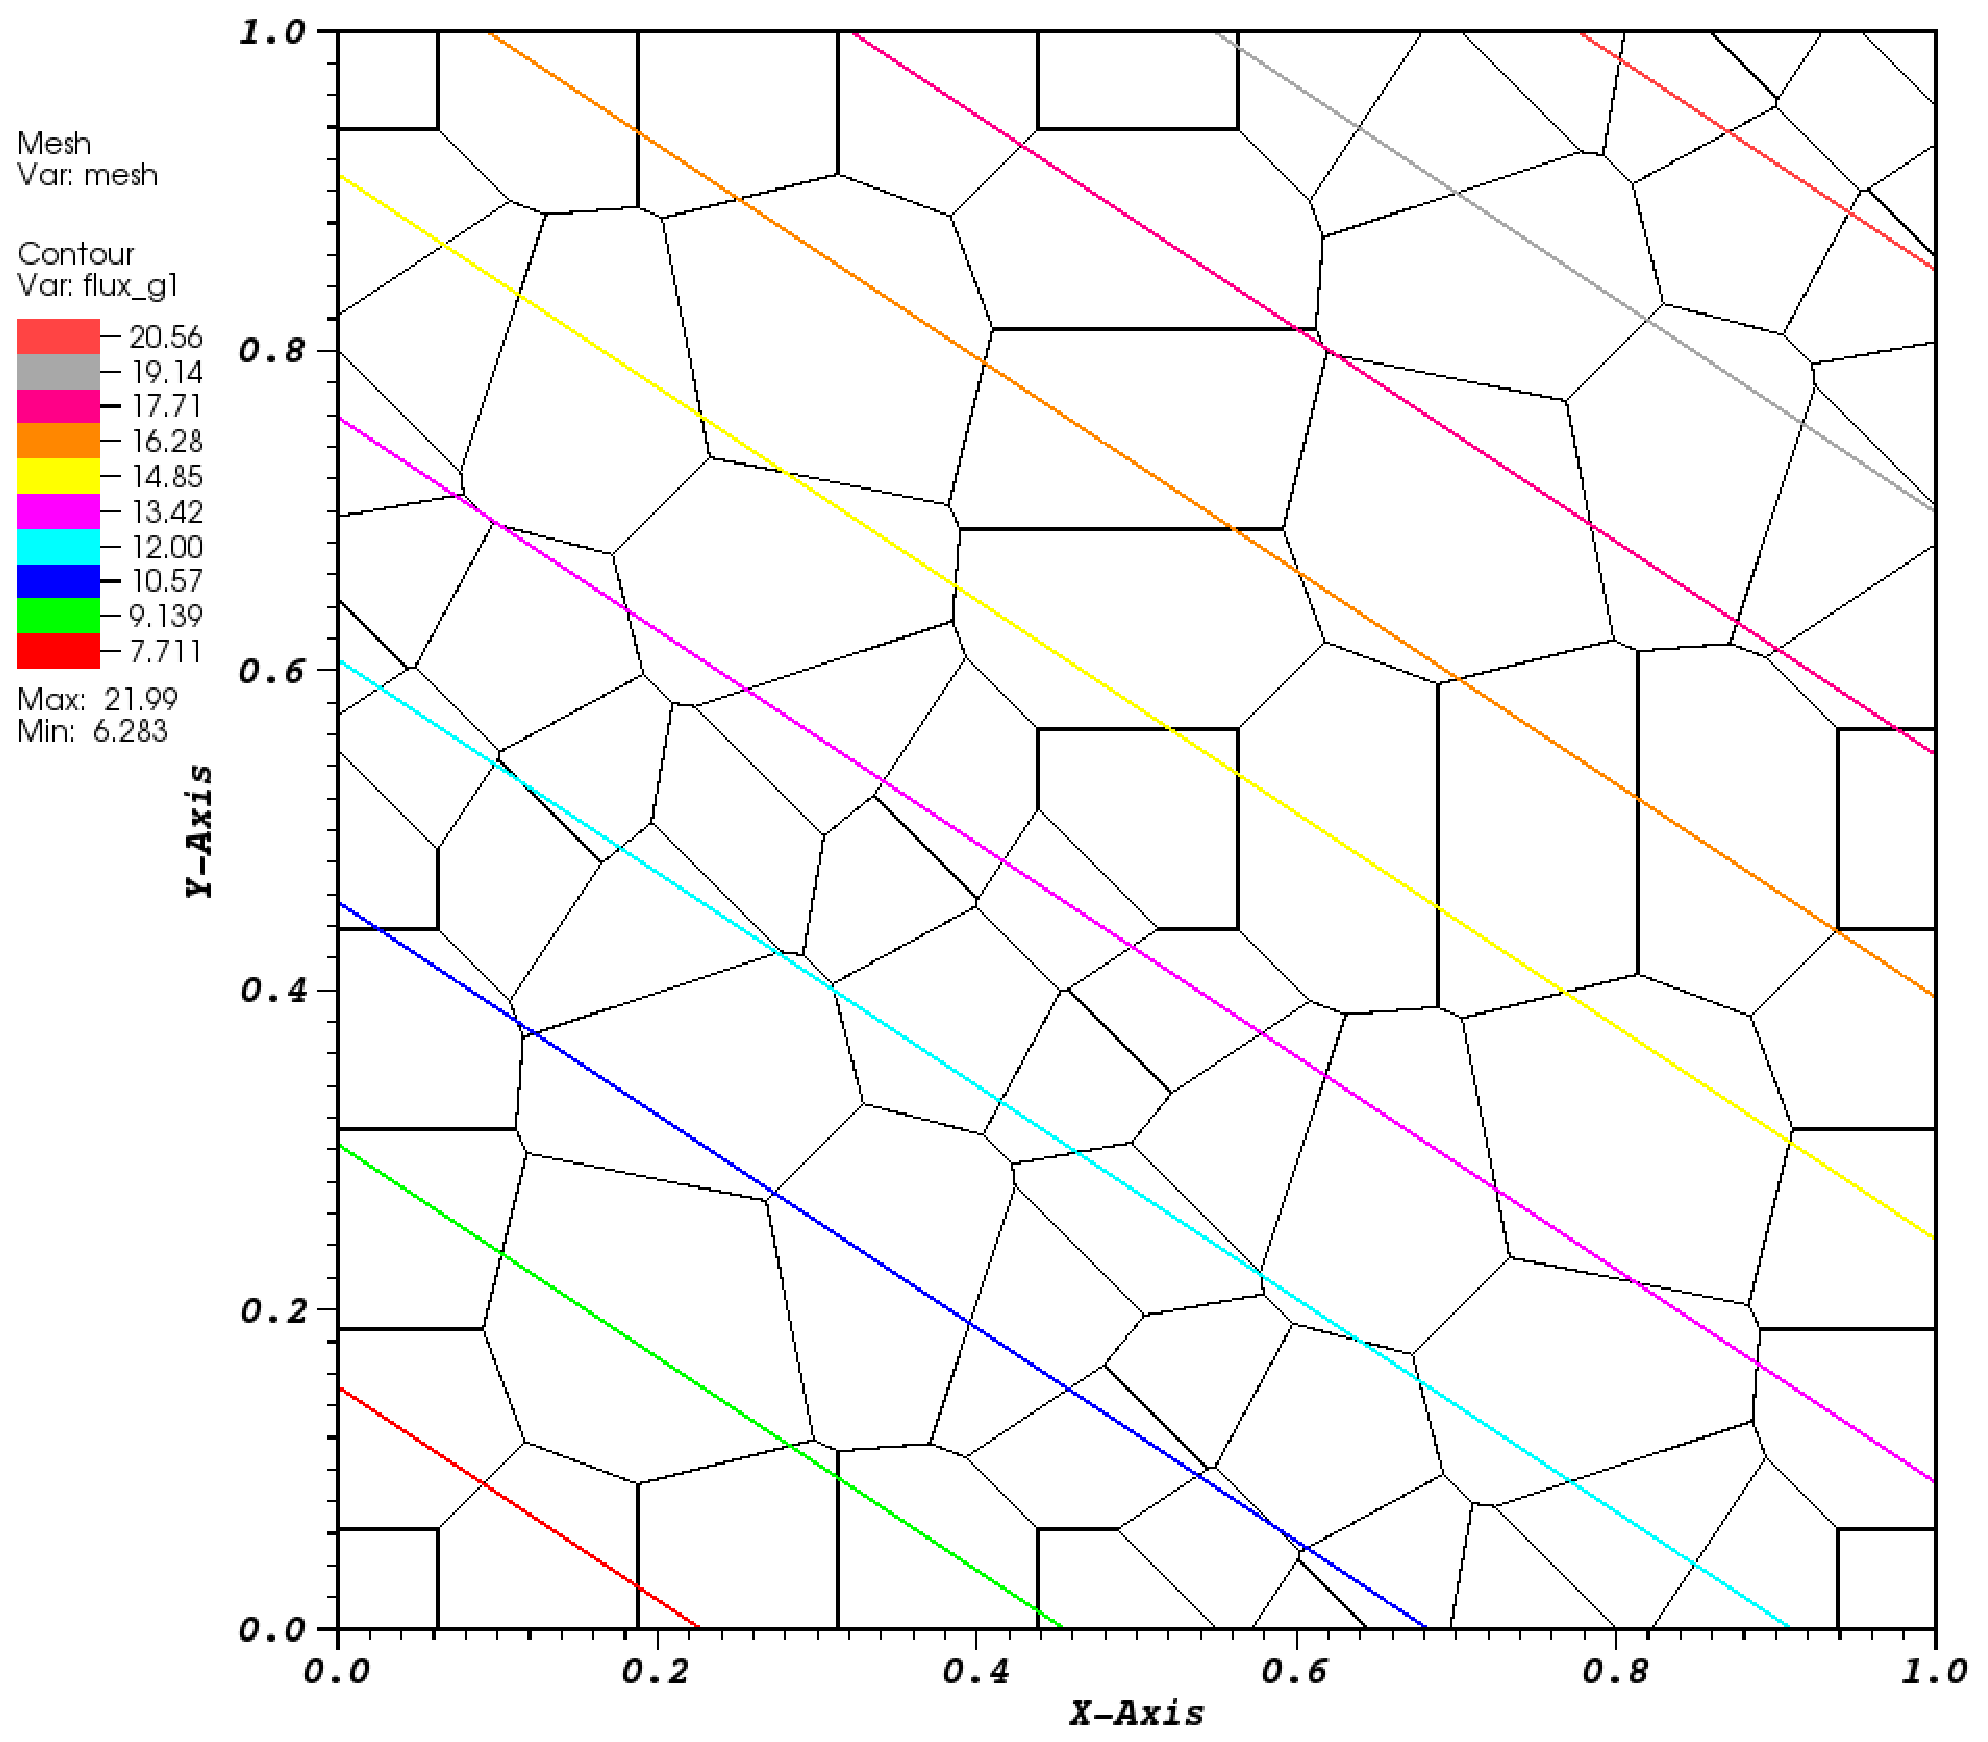
\includegraphics[width=\textwidth]{figures/smooth_poly_PWLD_k1.eps}
		\caption{}
	\end{subfigure}
	\hfill
	\begin{subfigure}[b]{0.42\textwidth}
		\centering
		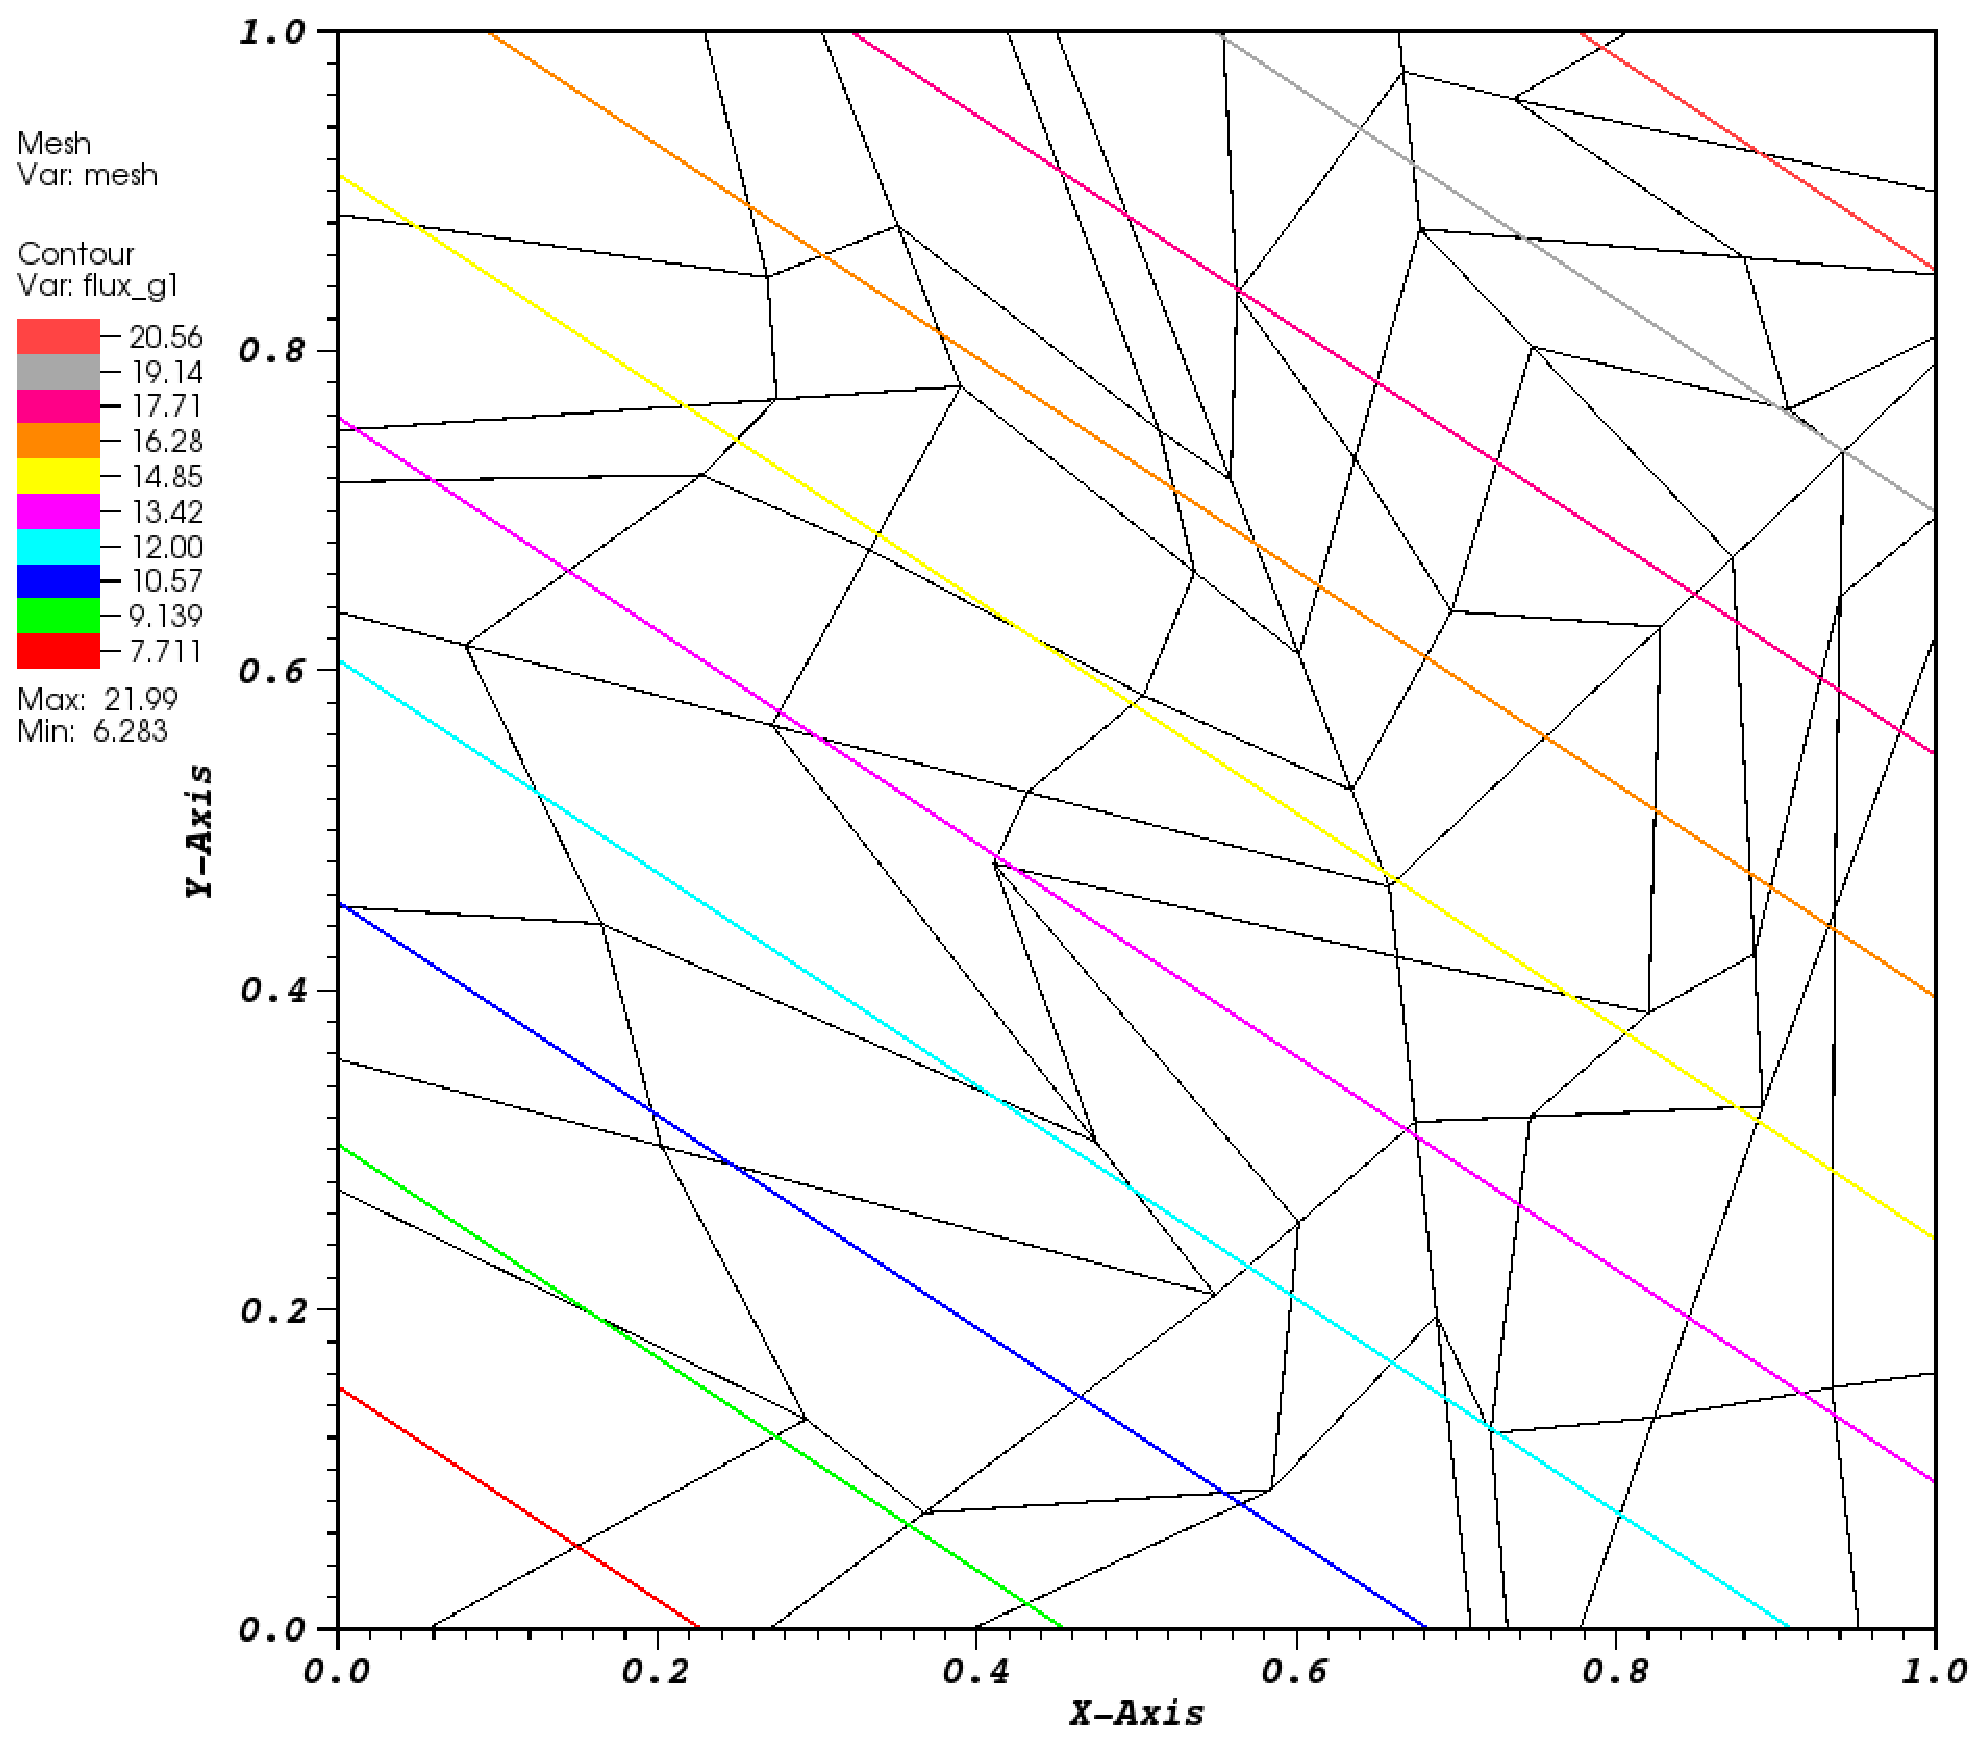
\includegraphics[width=\textwidth]{figures/shes_quad_PWLD_k1.eps}
		\caption{}
	\end{subfigure}
\caption{Exactly linear transport solutions using the PWL coordinates on (a) a sinusoidal polygonal mesh and (b) a highly-distorted quadrilateral shestakov mesh.}
\label{fig::lin_sol}
\end{figure}
\vspace{2mm}

We next want to analyze the convergence rate properties of transport solutions using the different basis functions on polygonal meshes. We will do this by use of the method of manufactured solutions (MMS) \cite{salari2000code}. We will use two different functional forms. First, we analyze a smoothly varying, $C^{\infty}$ analytical solution of the form,

\begin{equation}
\label{eq::sin_eq}
\begin{aligned}
	\Psi(x,y) = &\sin (\nu \frac{\pi x}{L_x}) \sin (\nu \frac{\pi y}{L_y}), \\
	\Phi(x,y) = 2 \pi &\sin (\nu \frac{\pi x}{L_x}) \sin (\nu \frac{\pi y}{L_y}),
\end{aligned}
\end{equation}

\noindent where in this case, the frequency parameter, $\nu$, is set to 3. We test the convergence rates of this transport solution using more regular meshes: orthogonal quadrilaterals, ordered triangles, and regular polygons. Figure \ref{fig::mms_err} presents the convergence rates 

We also wish to test a solution that contains an extreme local maximum. We analyze an analytical solution that contains a local gaussian function of the form,

\begin{equation}
\label{eq::gauss_eq}
\begin{aligned}
	\Psi (x,y) = & C_M x (L_x - x) y (L_y - y) \exp(-\frac{(x-x_0)^2 + (y-y_0)^2}{\gamma}) \\ 
	\Phi (x,y) = 2 \pi & C_M x (L_x - x) y (L_y - y) \exp(-\frac{(x-x_0)^2 + (y-y_0)^2}{\gamma})
\end{aligned} \, ,
\end{equation}

\noindent where the equation constant and the deviation parameter are

\begin{equation}
\label{eq::gaussconsts}
C_M = \frac{100}{L_x^2 L_y^2} \qquad \text{and} \qquad \gamma = \frac{L_x L_y}{100} ,
\end{equation}

\noindent respectively. However, for this transport solution, we will utilize adaptive mesh refinement strategies to test a different methodology in generating polygonal meshes. Figure \ref{fig::Gauss_AMR_err} contains some convergence rate analysis for the different linear basis functions and the quadratic maximu entropy coordinates. We then show the mesh refinement level and the corresponding localized gaussian solution in Figure \ref{fig::AMR_plots} for the both the linear and quadratic serendipity maximum entropy coordinates.

\begin{figure}[hbt]
\centering
	\begin{subfigure}[b]{0.485\textwidth}
		\centering
		\includegraphics[width=\textwidth]{figures/cart_err_rev1.eps}
		\caption{}
	\end{subfigure}
	\hfill
	\begin{subfigure}[b]{0.49\textwidth}
		\centering
		\includegraphics[width=\textwidth]{figures/poly_err_rev1.eps}
		\caption{}
	\end{subfigure}
\caption{$L_2$ error norm for the sinusoidal MMS problem using the various 2D polygonal basis functions on (a) orthogonal quadrilateral meshes and (b) random polygonal meshes.}
\label{fig::mms_err}
\end{figure}

\begin{figure}[!hbt]
\centering
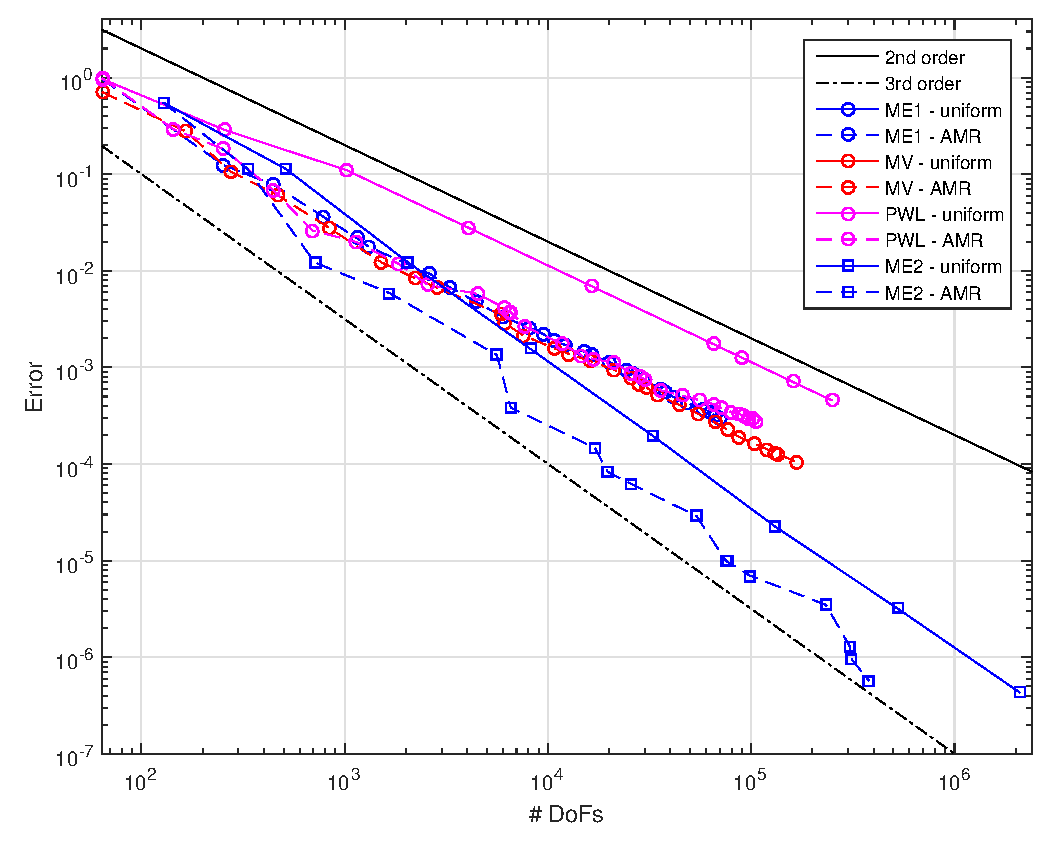
\includegraphics[width=0.6\textwidth]{figures/Transport_Gauss_2D_AMR_Error_Plot.eps}
\caption{$L_2$ error norm for the gaussian MMS problem using the various 2D polygonal basis functions }
\label{fig::Gauss_AMR_err}
\end{figure}

\begin{figure}[hbt]
\centering
	\begin{subfigure}[b]{0.35\textwidth}
		\centering
		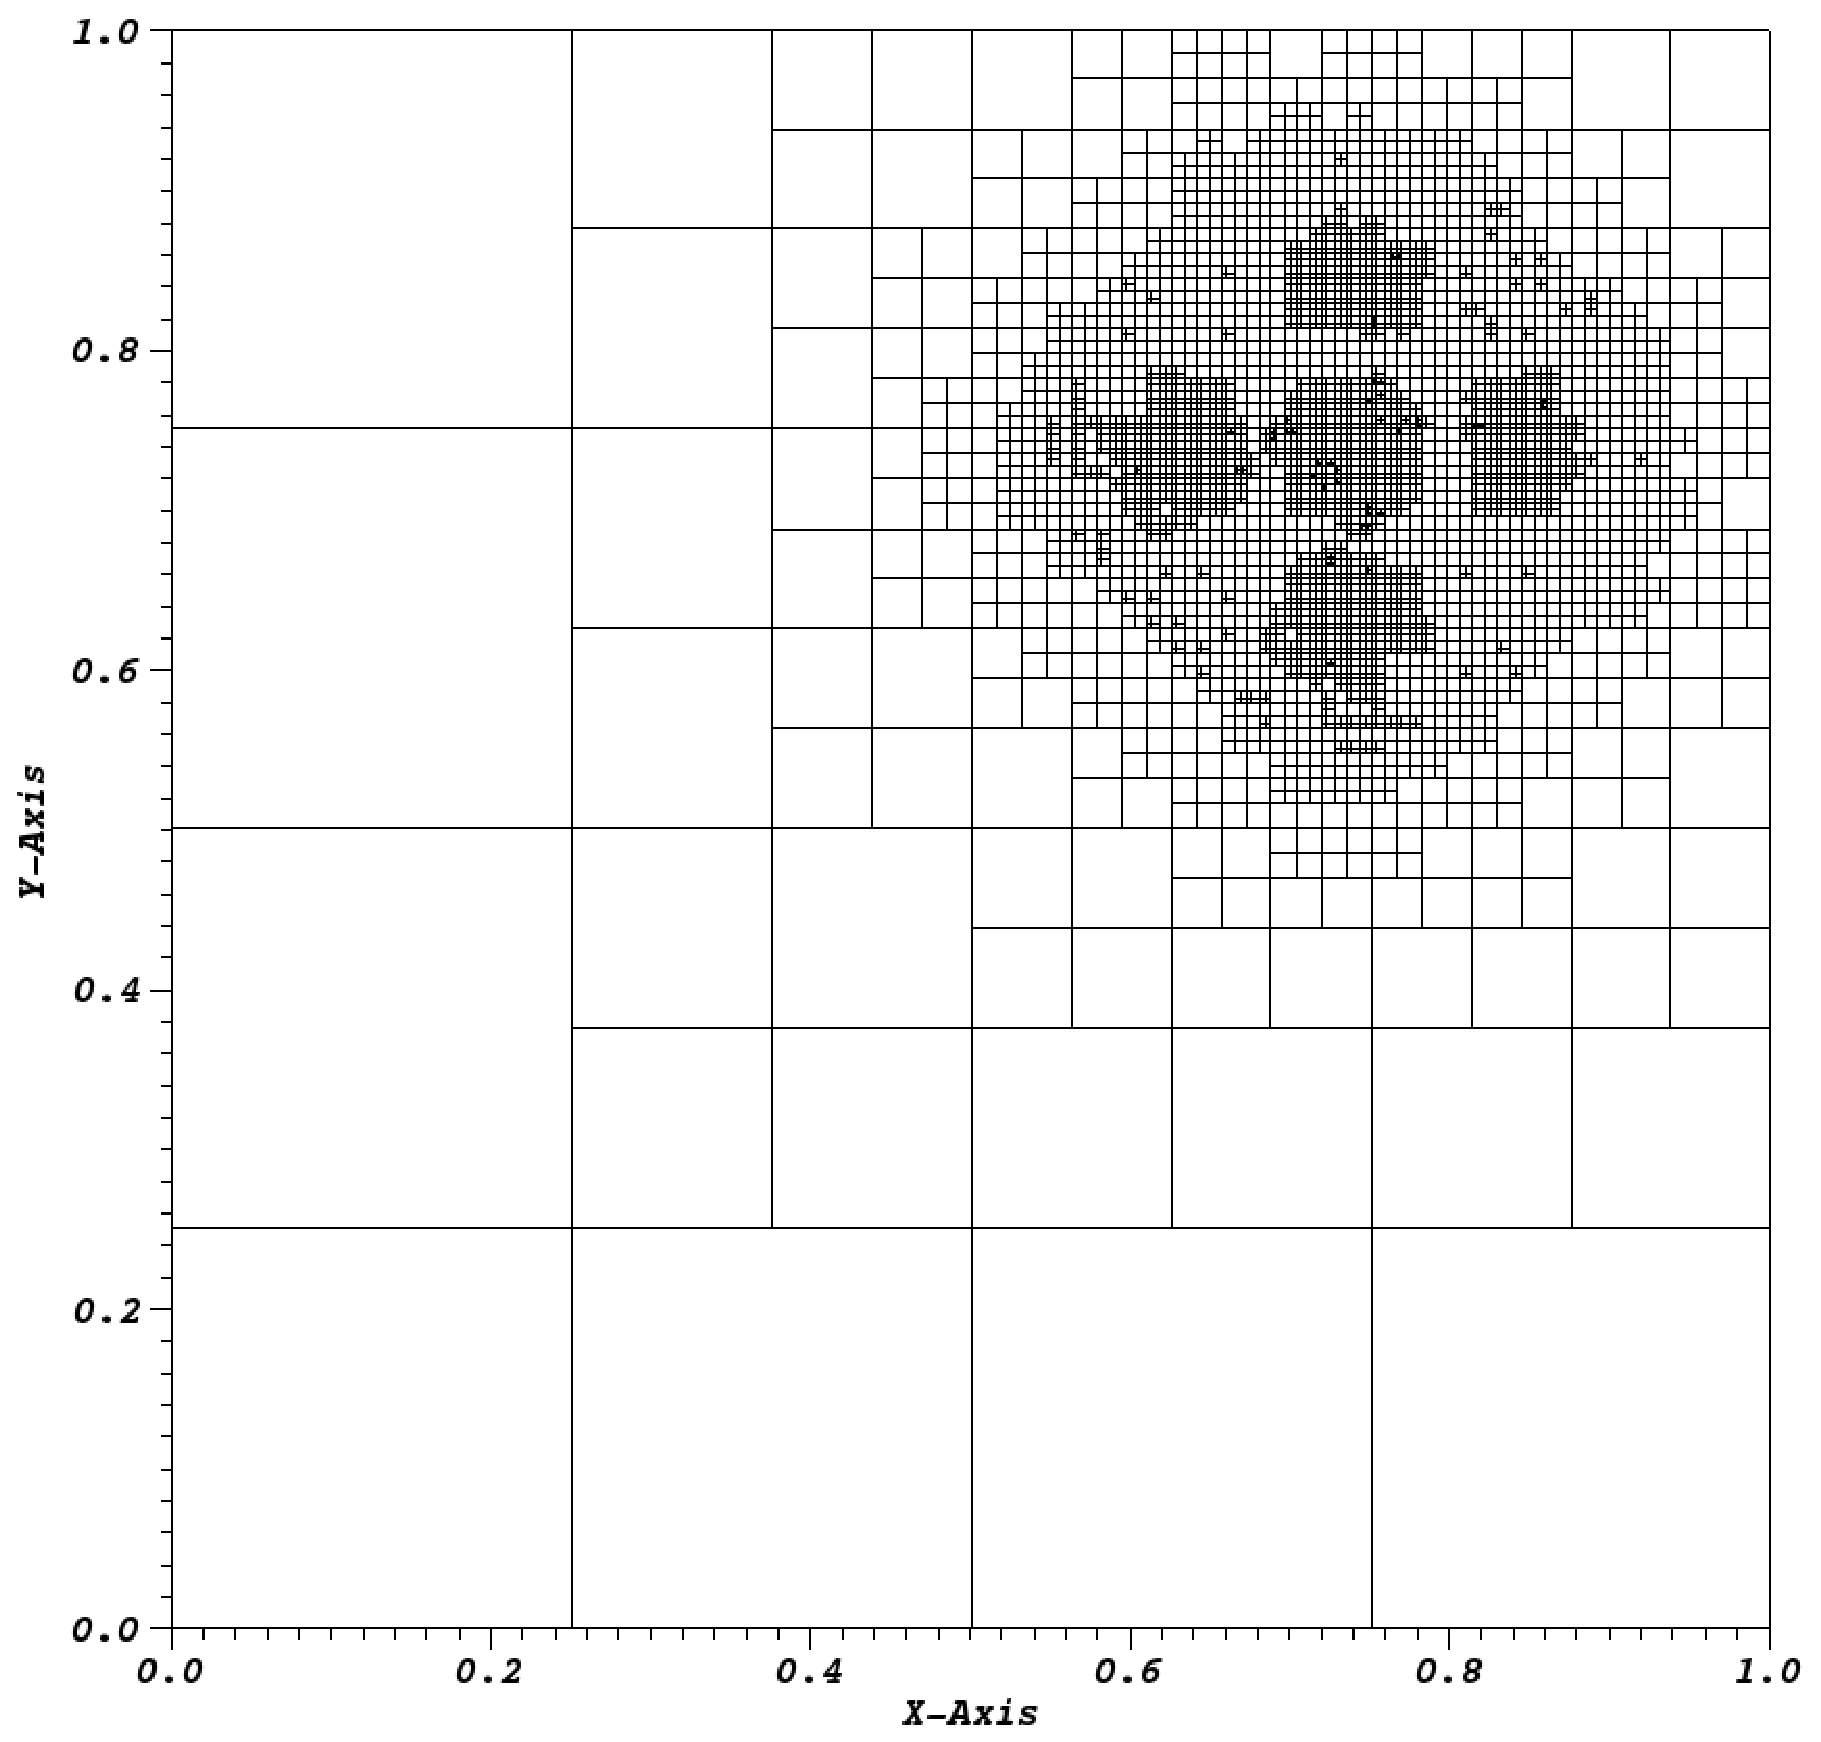
\includegraphics[width=\textwidth]{figures/ME1_cart_mesh.eps}
	\end{subfigure}
	\hspace{1cm}
	\begin{subfigure}[b]{0.35\textwidth}
		\centering
		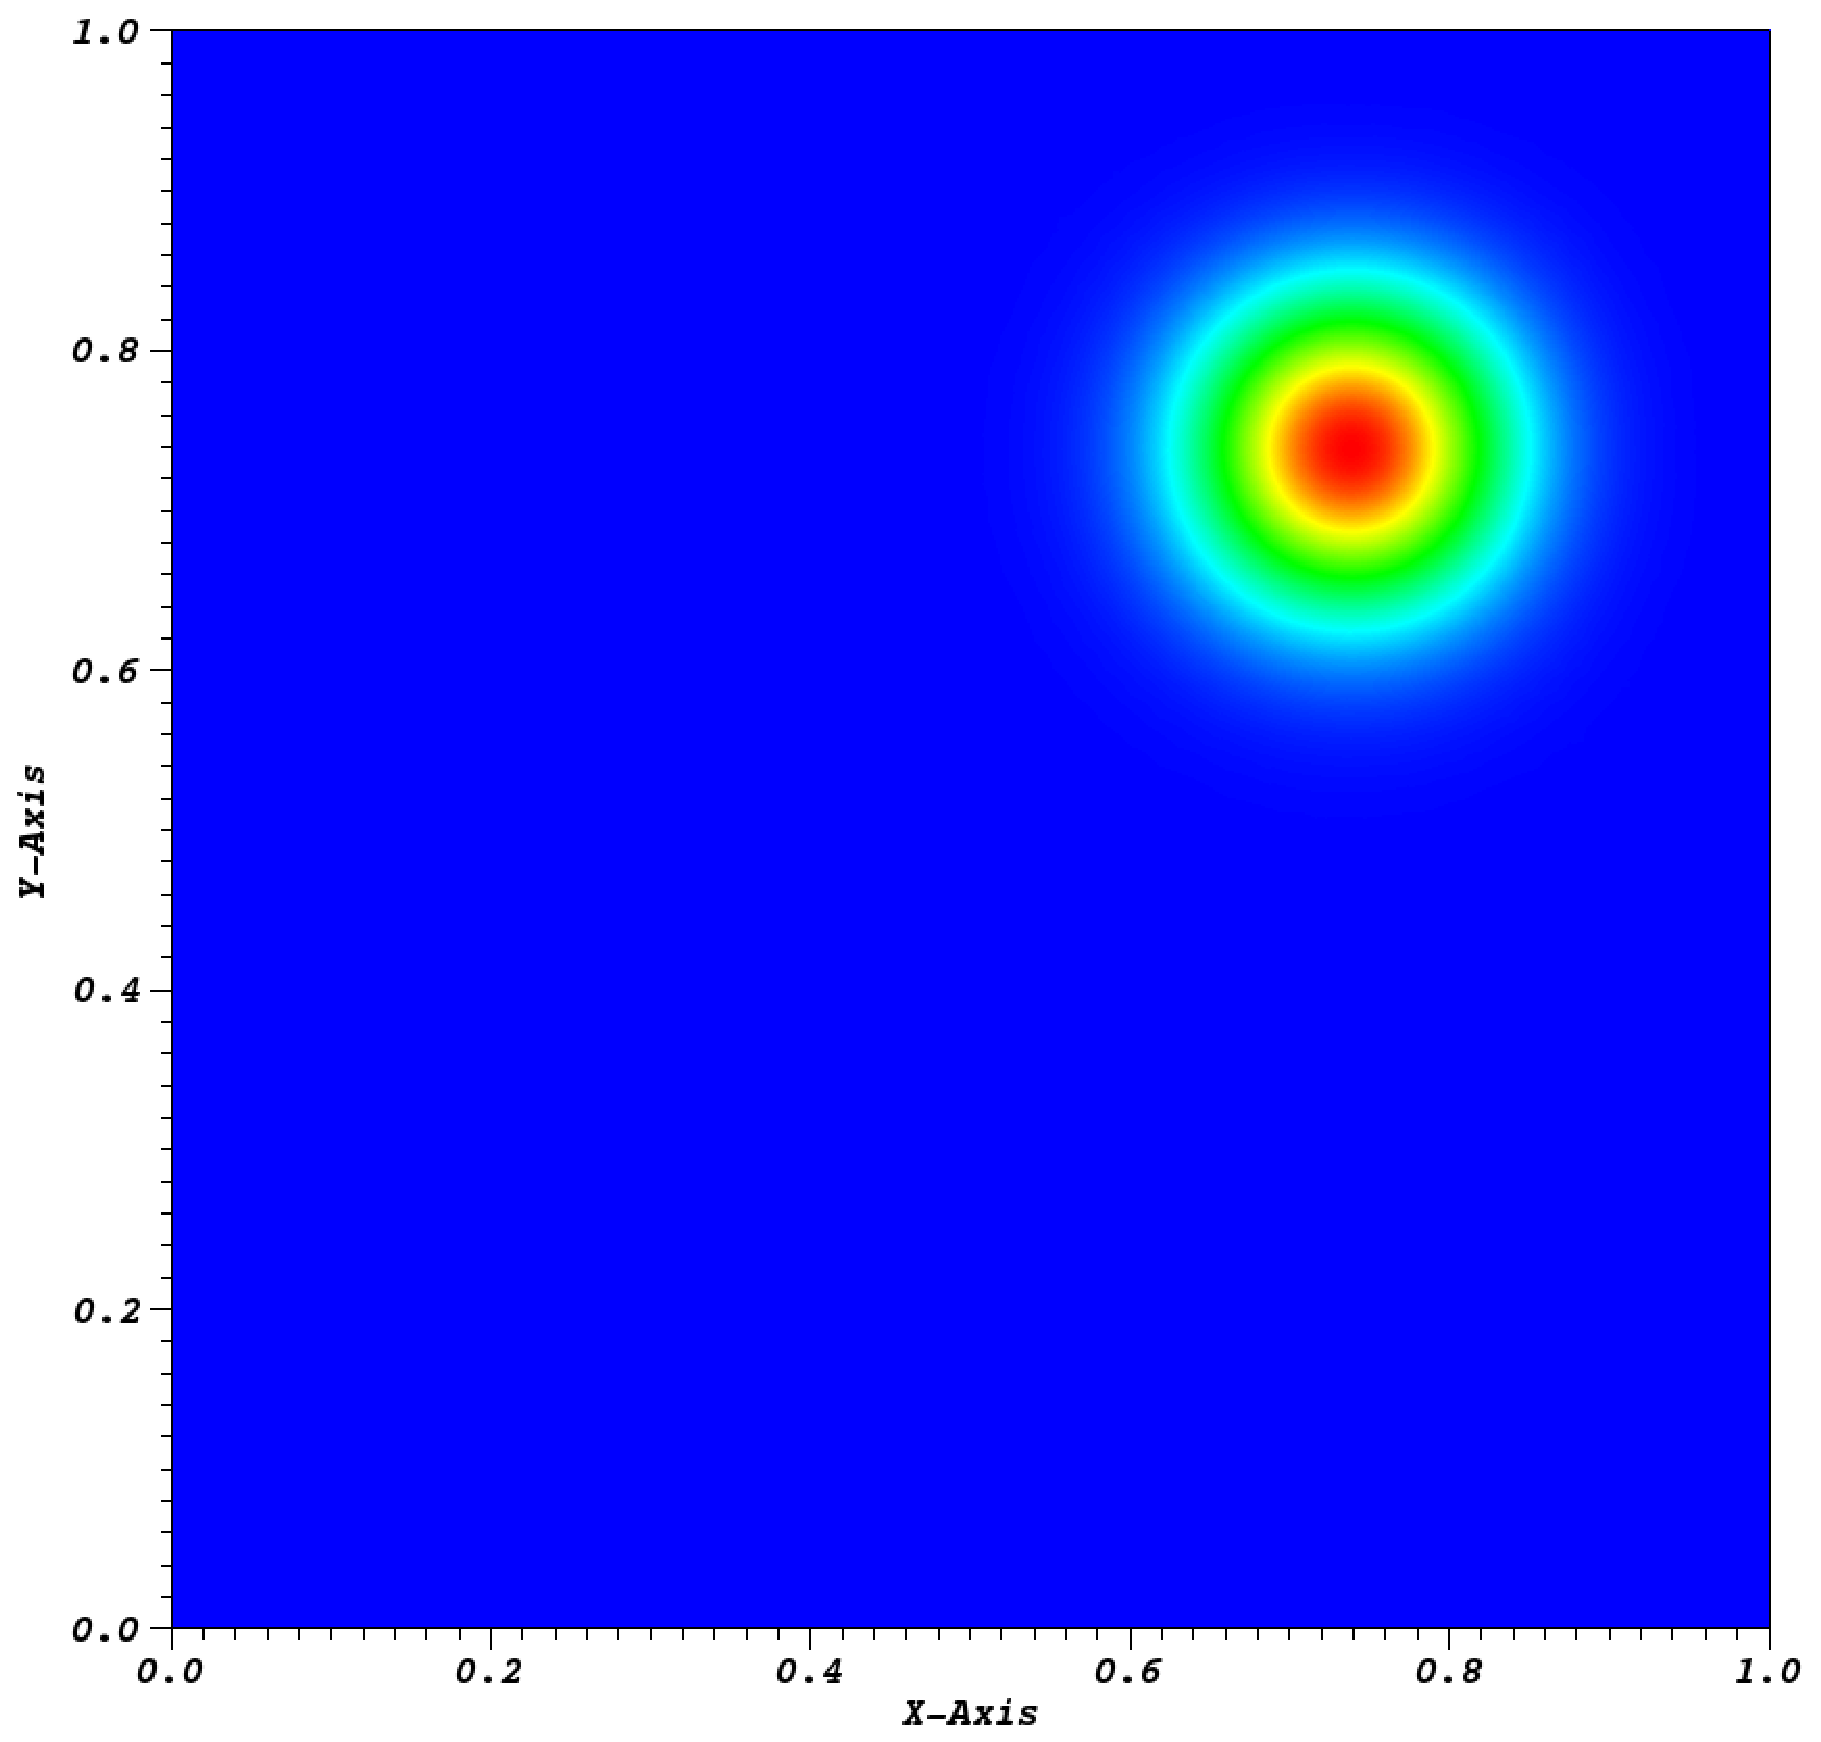
\includegraphics[width=\textwidth]{figures/ME1_cart_sol.eps}
	\end{subfigure}
	\par\bigskip
	\begin{subfigure}[b]{0.35\textwidth}
		\centering
		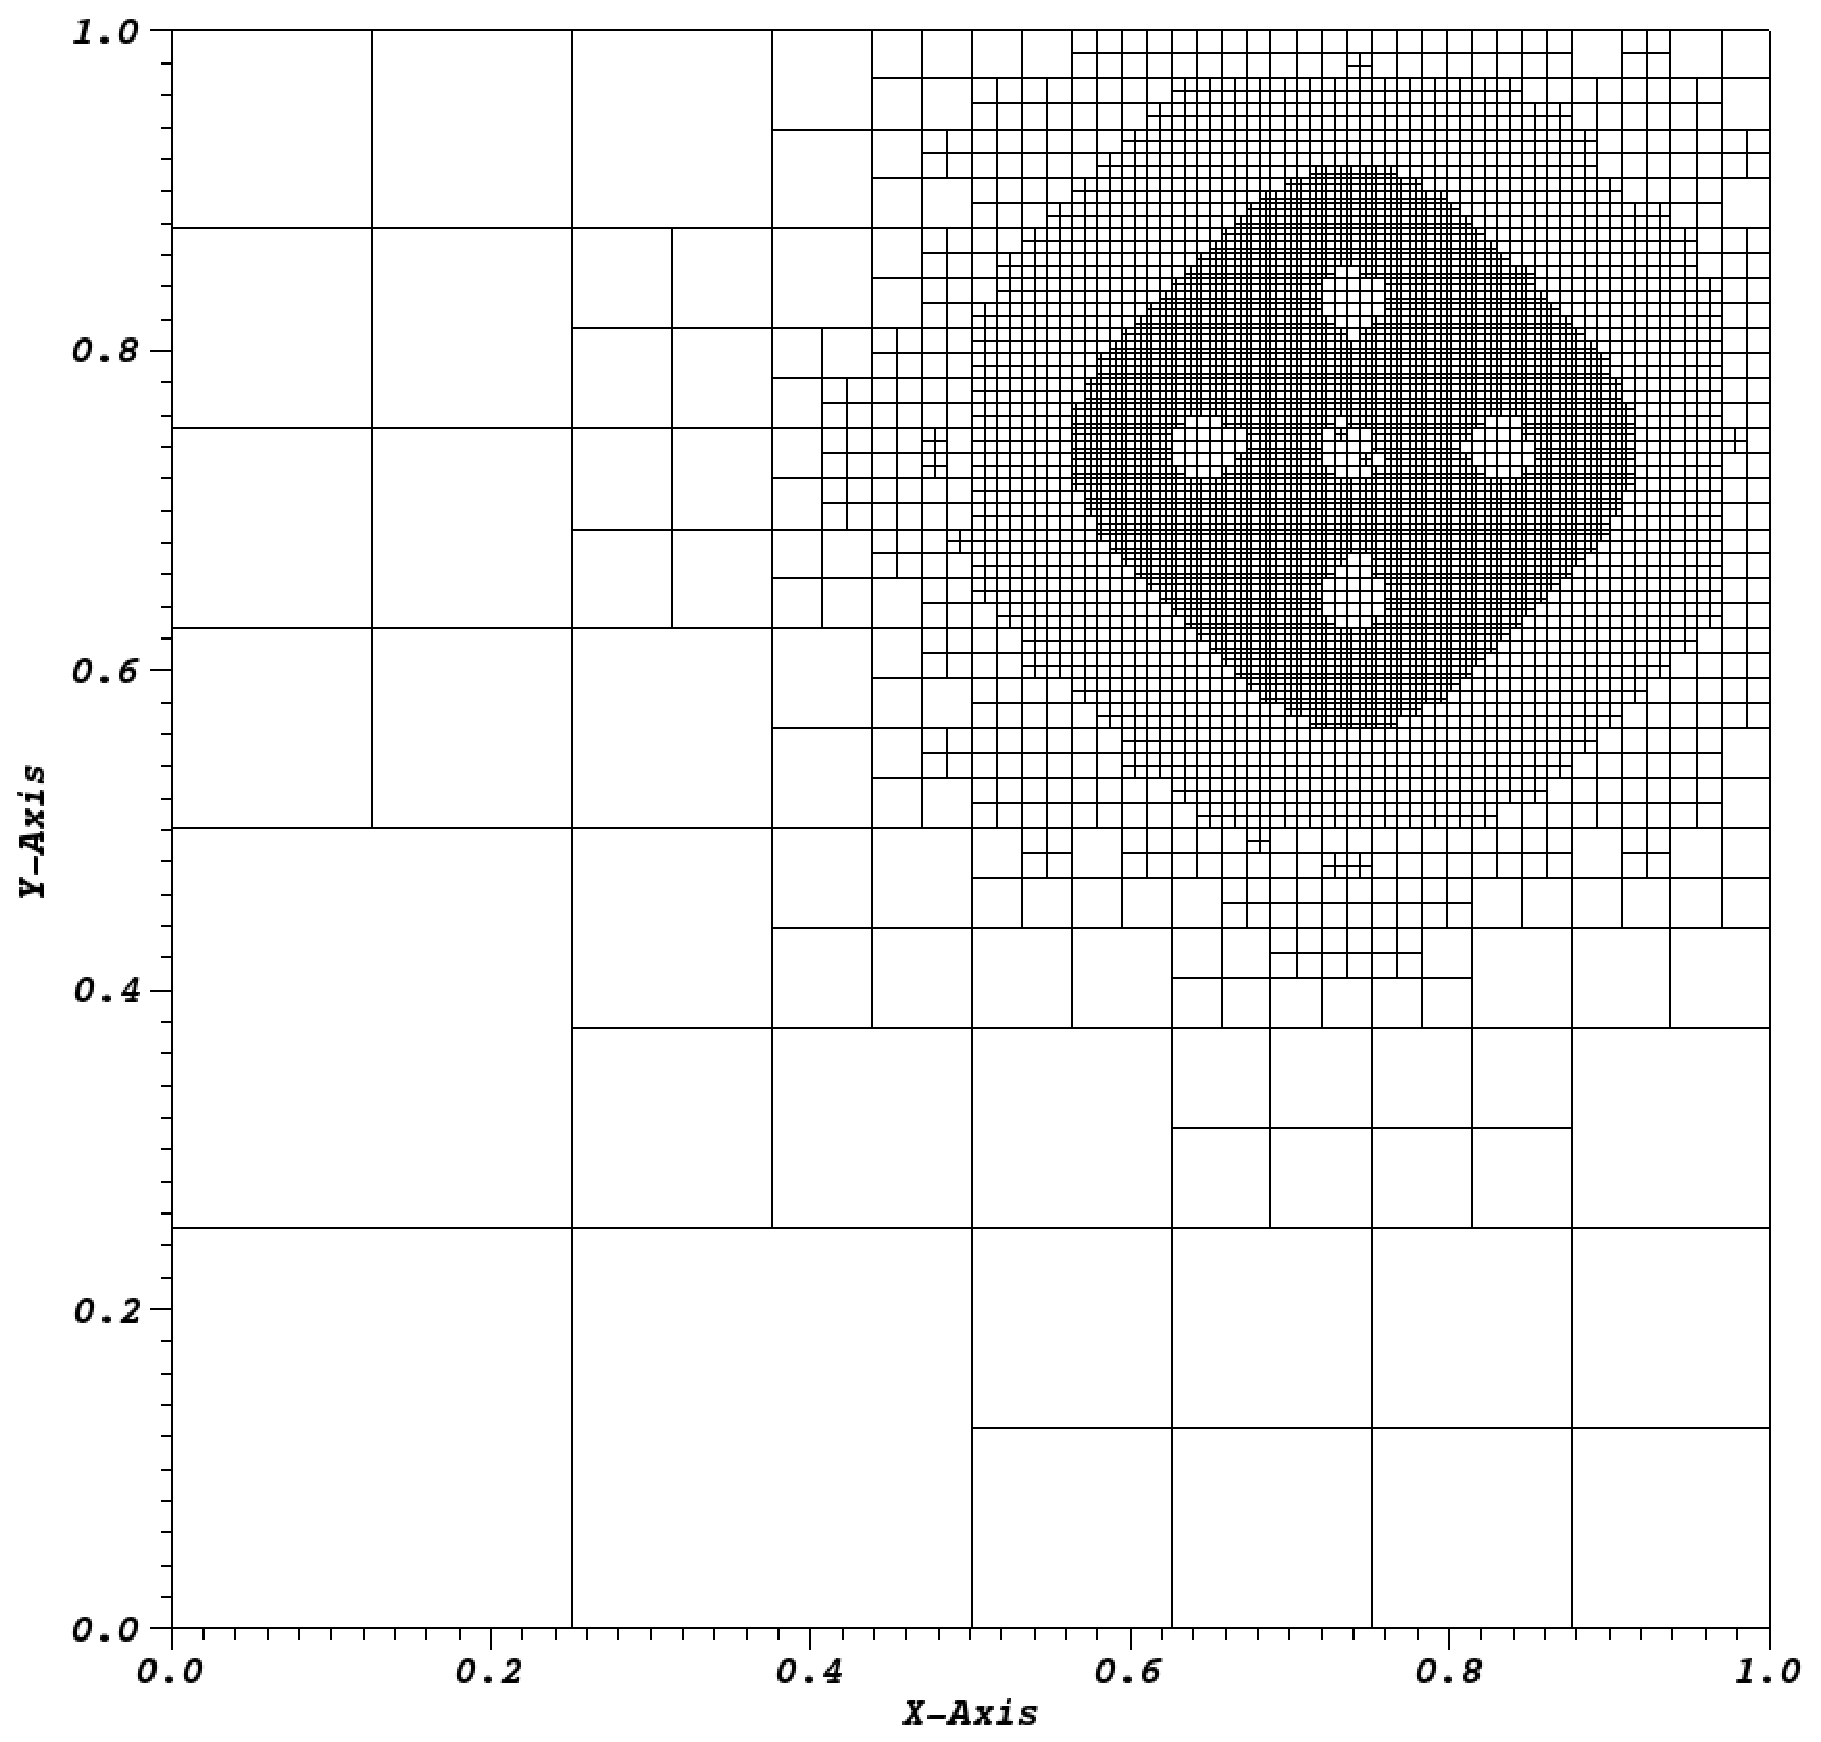
\includegraphics[width=\textwidth]{figures/ME2_cart_mesh.eps}
	\end{subfigure}
	\hspace{1cm}
	\begin{subfigure}[b]{0.35\textwidth}
		\centering
		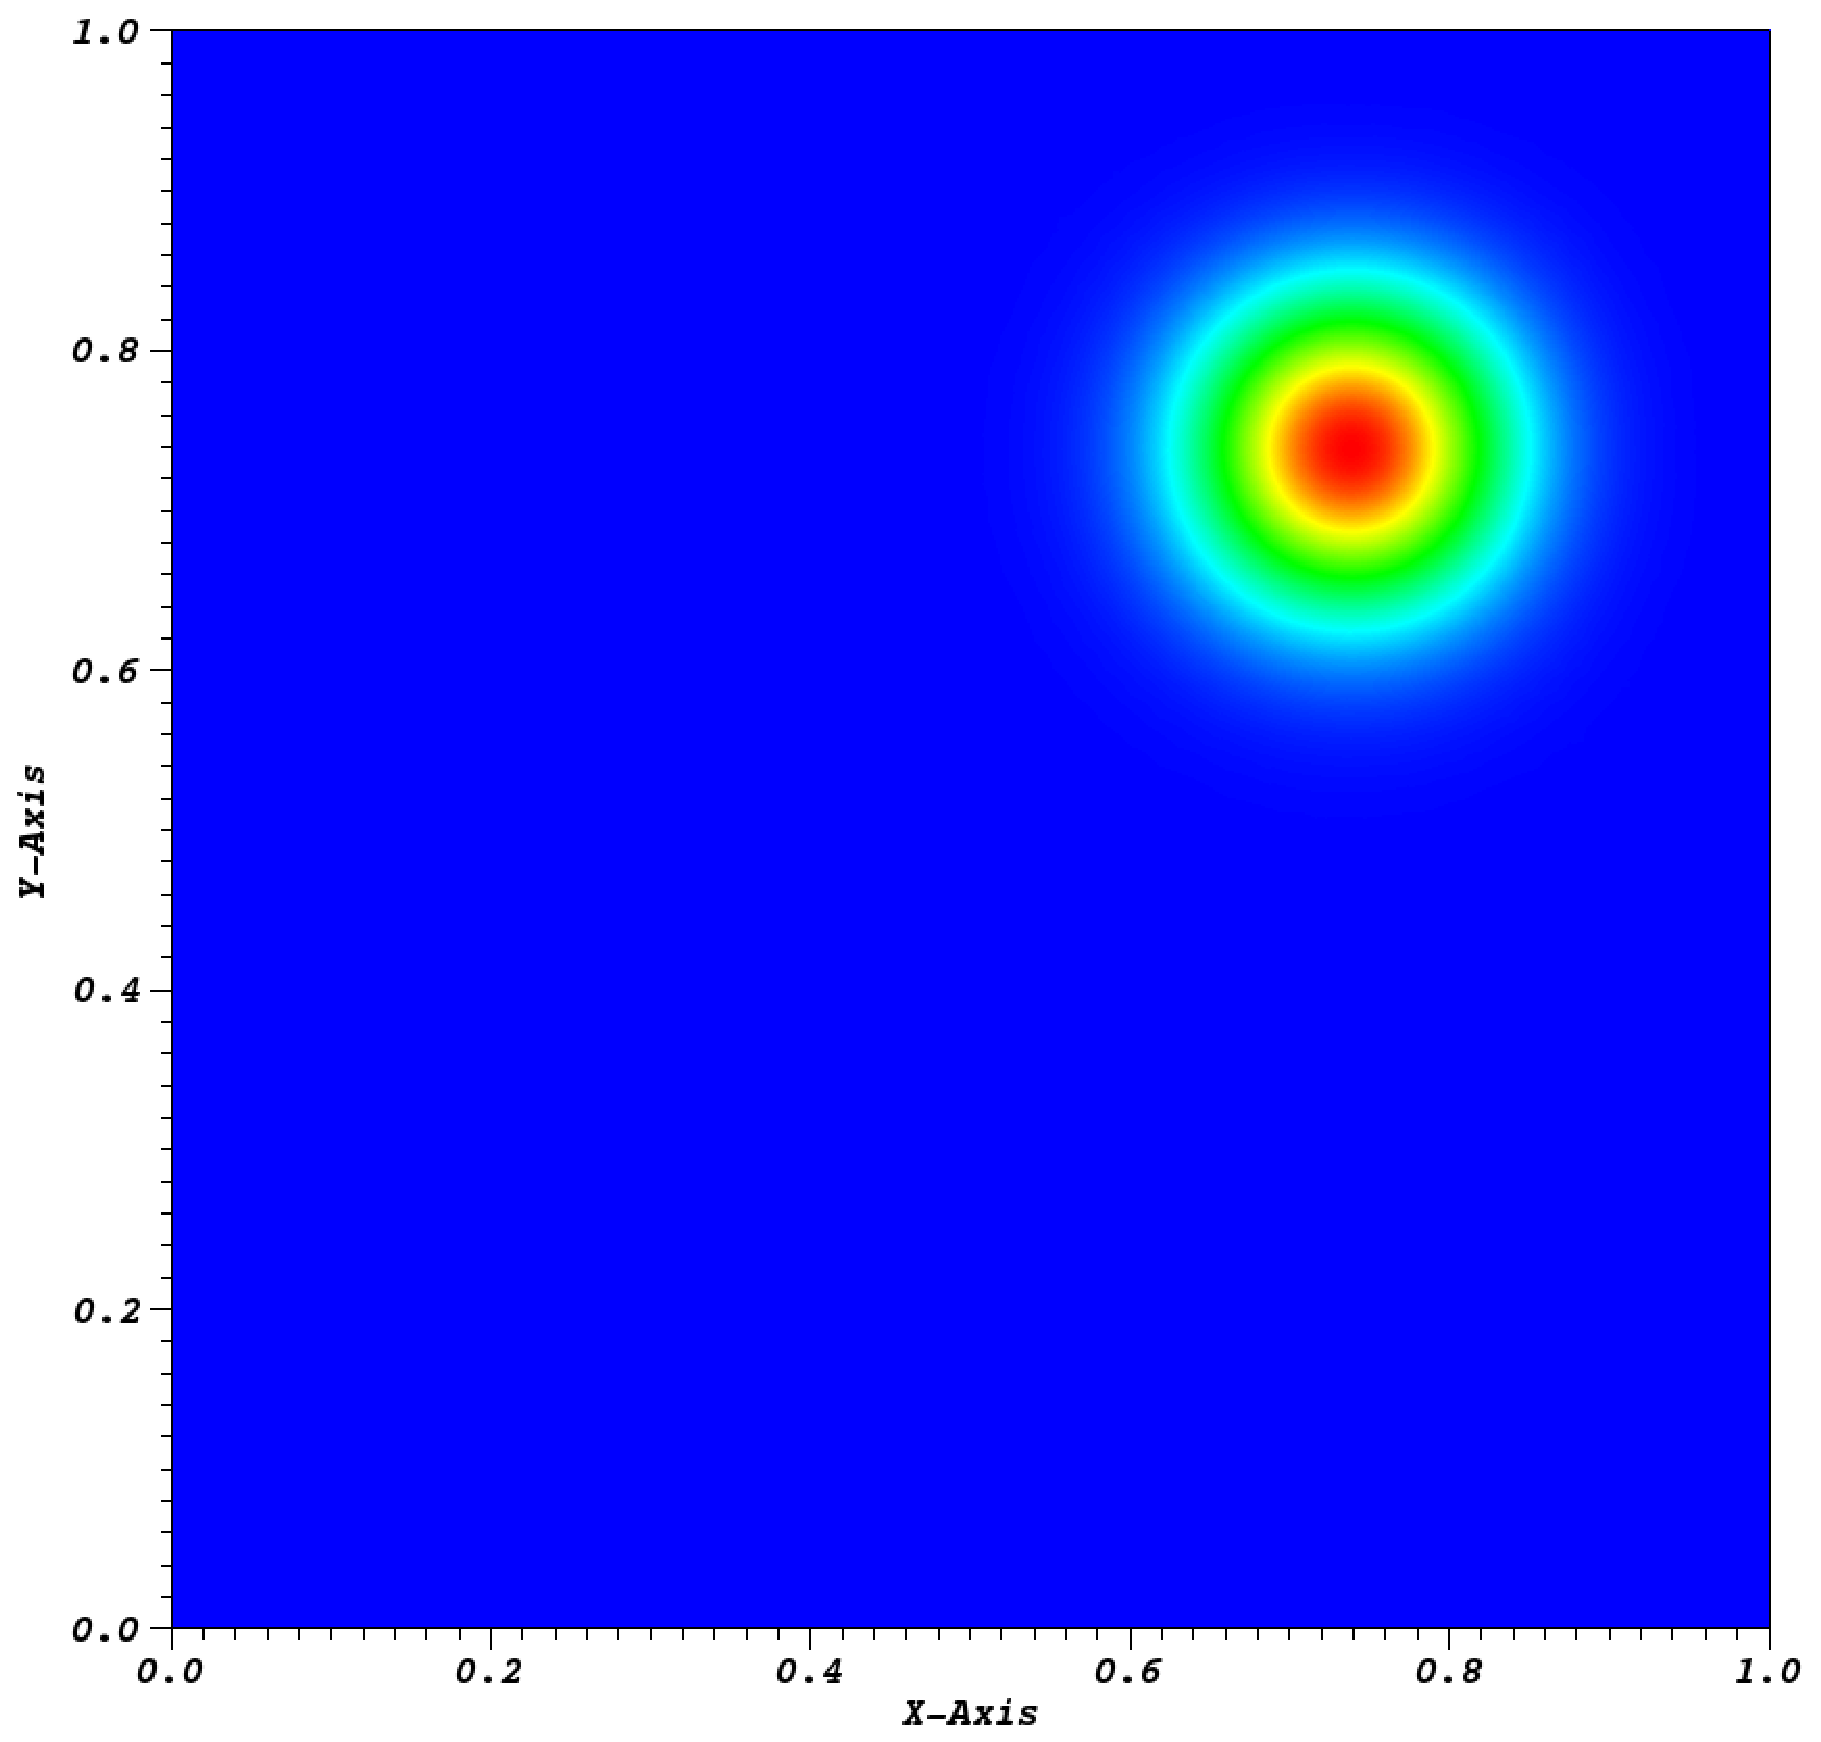
\includegraphics[width=\textwidth]{figures/ME2_cart_sol.eps}
	\end{subfigure}
\caption{AMR meshes and solution plots using the linear maximum entropy coordinates at cycle 15 (top) and the quadratic serendipity maximum entropy coordinates at cycle 08 (bottom).}
\label{fig::AMR_plots}
\end{figure}

%%%%%%%%%%%%%%%%%%%%%%%%%%%%%%%%%%%%%%%%%%%%%%%%%%%%%%%%%%%%%%%%%%%%%%
\subsection{Diffusion Synthetic Acceleration for Massively-Parallel Problems}
\label{sec::CW_DSA}

The second topical area of research for this dissertation work will focus on the use of DSA schemes to precondition the transport operators for massively-parallel problems.

As it was previously stated, efficient methods for inverting the streaming operator do not guarantee efficiency in solving the transport problem for optically thick configurations. We recast the discretized transport equation from Eq. (\ref{eq::trans_eq}):

\begin{equation}
\label{eq::CW_trans_eq}
\begin{aligned}
{\bf A} \Psi &= {\bf B} \Phi +  {\bf C} \Phi + {\bf Q} \\
\Phi &= {\bf D} \Psi
\end{aligned} ,
\end{equation}

\noindent where ${\bf A}$, ${\bf B}$, ${\bf C}$, and ${\bf Q}$ are different operators of the transport problem. We then define an iterative procedure of the form,

\begin{equation}
\label{eq::CW_trans_eq_it}
{\bf A} \Psi^{(k+1/2)} = {\bf B} \Phi^{(k+1/2)} + {\bf C} \Phi^{(k)} + {\bf Q},
\end{equation}

\noindent where ${\bf B}$ operates on the current solution iterate and ${\bf C}$ operates on the previous solution iterate. We then subtract Eq. (\ref{eq::CW_trans_eq_it}) from Eq. (\ref{eq::CW_trans_eq}) to yield the following formulation of the solution error at iterate $(k+1/2)$,

\begin{equation}
\label{eq::CW_trans_eq_it_diff}
{\bf A} \delta \Psi^{(k+1/2)} - {\bf B}' \delta \Phi^{(k+1/2)} = {\bf R}^{(k+1/2)}, 
\end{equation}

\noindent where
\begin{equation}
\label{eq::CW_delta_fluxes}
\begin{aligned}
\delta \Psi^{(k+1/2)} &\equiv  \Psi - \Psi^{(k+1/2)} \\
\delta \Phi^{(k+1/2)} &\equiv {\bf D} \delta \Psi^{(k+1/2)}
\end{aligned} \, ,
\end{equation}

\noindent are the errors in the angular fluxes and flux moments, ${\bf R}^{(k+1/2)}$ is some residual in the error, and the operators ${\bf B}$ and ${\bf B'}$ are not necessarily the same. If we could exactly solve for the error in Eqs. (\ref{eq::CW_trans_eq_it_diff} - \ref{eq::CW_delta_fluxes}), then the exact solution could be calculated by: $\Phi =  \Phi^{(k+1/2)} + \delta \Phi^{(k+1/2)}$. Unfortunately, Eq. (\ref{eq::CW_trans_eq_it_diff}) is just as difficult to solve as Eq. (\ref{eq::CW_trans_eq}). Therefore, we estimate Eq. (\ref{eq::CW_trans_eq_it_diff}) with a low-order operator that is easy to solve. We will next briefly described the low-order operator that we will utilize in Section \ref{sec::CW_DSA_MIP}.


%%%%%%%%%%%%%%%%%%%
\subsubsection{Modified Interior Penalty Diffusion Form for DSA Preconditioning}
\label{sec::CW_DSA_MIP}

As previously stated in Section \ref{sec::PS}, the diffusion operator has been utilized in different forms for the low-order operators of Eq. (\ref{eq::CW_trans_eq_it_diff}). As mentioned, the MIP DSA form has many beneficial properties and it has been extensively analyzed for 2D transport problems \cite{ref::DSA_wang_ragusa,turcksin2014discontinuous}. In this dissertation work, we will extend the MIP DSA analysis to 3D transport problems. We will also extensively analyze its scalability for massively-parallel problems.

The MIP diffusion form is defined with the following bilinear left-hand-side,

\begin{equation}
\label{eq::mip_lhs}
\begin{aligned}
a(\delta \Phi, b)  = \Big<  D \vec{\nabla} \delta  \Phi , \vec{\nabla} b \Big>_{\mathcal{D}} + \Big<  \sigma \delta  \Phi , b  \Big>_{\mathcal{D}}    \\
+  \Big\{ \kappa_e^{MIP} [\![ \delta  \Phi ]\!] , [\![  b ]\!]\Big\}_{E_h^i} + \Big\{  [\![  \delta \Phi ]\!] , \{\!\{  D \partial_n b \}\!\}\Big\}_{E_h^i}  + \Big\{ \{\!\{  D \partial_n \delta \Phi \}\!\} , [\![ b ]\!]\Big\}_{E_h^i} \\
+ \Big\{ \kappa_e^{MIP}  \delta \Phi ,   b \Big\}_{\partial \mathcal{D}^{vac}} - \frac{1}{2} \Big\{  \delta \Phi  ,  D \partial_n b \Big\}_{\partial \mathcal{D}^{vac}} - \frac{1}{2} \Big\{   D \partial_n \delta  \Phi , b \Big\}_{\partial \mathcal{D}^{vac}}  
\end{aligned} ,
\end{equation}

\noindent and with the following linear right-hand-side,

\begin{equation}
\label{eq::mip_rhs}
\ell(b) = \Big<  R, b  \Big>_{\mathcal{D}} + \Big\{ \delta  J^{inc}, b \Big\}_{\partial \mathcal{D}^{ref}} .
\end{equation}

\noindent The MIP penalty coefficient, $\kappa_e^{MIP}$, has the form:

\begin{equation}
\label{eq::ip_penalty}
\kappa_e^{MIP} = \max(\frac{1}{4}, \kappa_e^{IP}) , \qquad
\kappa_e^{IP}  \equiv 
		\begin{cases}
		\frac{C_B}{2} \left(  \frac{D^+}{h^+} + \frac{D^-}{h^-}  \right) & , e \in E_h^i \\
		C_B \frac{D^-}{h^-}  & , e \in \partial \mathcal{D}
		\end{cases} \, ,
\end{equation}

\noindent where $C_B=cp(p+1)$, $c$ is a user defined constant ($c \geq 1$), $p$ is the polynomial order of the basis function, $D^{\pm}$ are the diffusion coefficients on either side of face $e$ and $h^{\pm}$ are the orthogonal projections on either side of face $e$. We determine the positive and negative cells by the following trace:

\begin{equation}
\label{eq::mip_trace}
u^{\pm} = \lim_{s \rightarrow 0^{\pm}} u (\vec{r} + s \vec{n}) .
\end{equation}

\noindent For interior faces, we can specify an arbitrary direction for the face normal, but boundary faces require the face normals to orient outwards from the domain.

To date, we have carried out extensive analysis for both 2D and 3D MIP DSA preconditioning. This includes analyzing all the linear and quadratic serendipity polygonal coordinates using fourier analysis and comparing to numerical simulations. In addition, we have analyzed the theoretical effects of strong heterogenities in material cross sections as well the effects of the use of DSA in conjunction with AMR calculations. 

Much work has also been performed to utilize the MIP DSA scheme to accelerate large transport calculations. Figure \ref{fig::fourier_NSR} shows an extension of the MIP analysis to 3D hexahedral cells. We demonstrate through both fourier and numerical analysis that the MIP form is unconditionally stable and robust across the full spectrum of cell optical thicknesses. In addition, the form is stable for mesh cells with large aspect ratios. We have also implemented the MIP DSA method into the PDT code at Texas A\&M University. The code uses the HYPRE library to efficiently invert the system matrix using PCG with BoomerAMG as the preconditioner \cite{ref::hypre,yang2002boomeramg}. Timing results from a homogenized Zerr weak scaling problem are presented in Figure \ref{fig::Vulcan_MIP_Timing}. We can see that our acceleration implementation yields good scaling results with the HYPRE solves and DSA takes up about 50\%-60\% of the total solve at high processor counts. We further note that we ran only a coarse transport problem with S8 angular quadrature and 1 energy group. If more angles or energy groups are used for a larger problem, then the time spent in the DSA solves will become negligible.

\begin{figure}
\centering
	\begin{subfigure}[b]{0.48\textwidth}
		\centering
		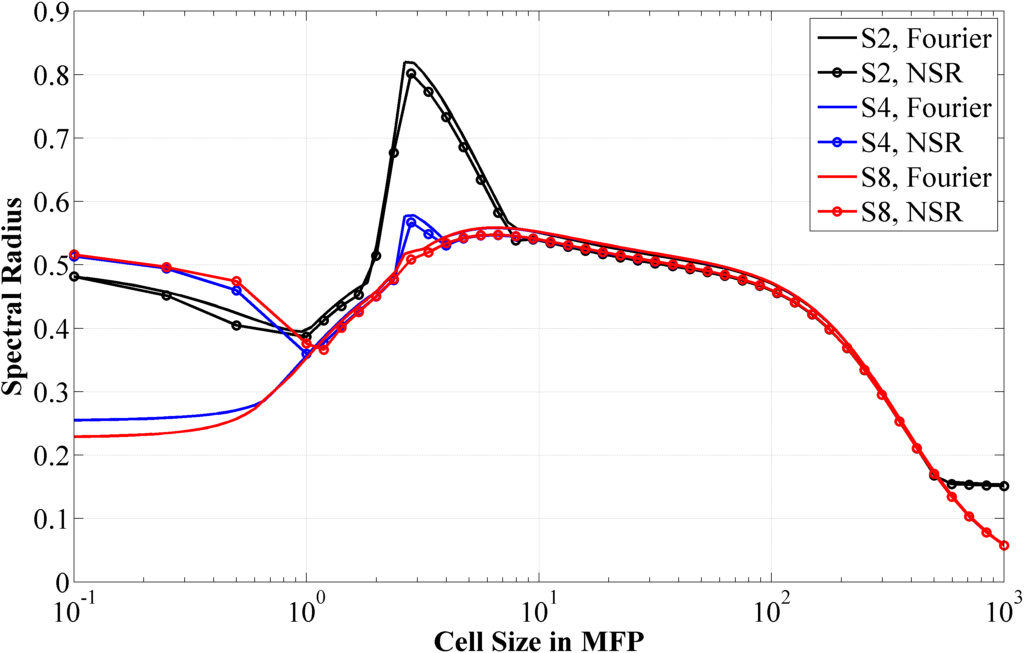
\includegraphics[width=\textwidth]{figures/SI_MIP_hex_C=1_LS2,4,8_F&NSR_PDT.png}
	\end{subfigure}
	\hfill
	\begin{subfigure}[b]{0.48\textwidth}
		\centering
		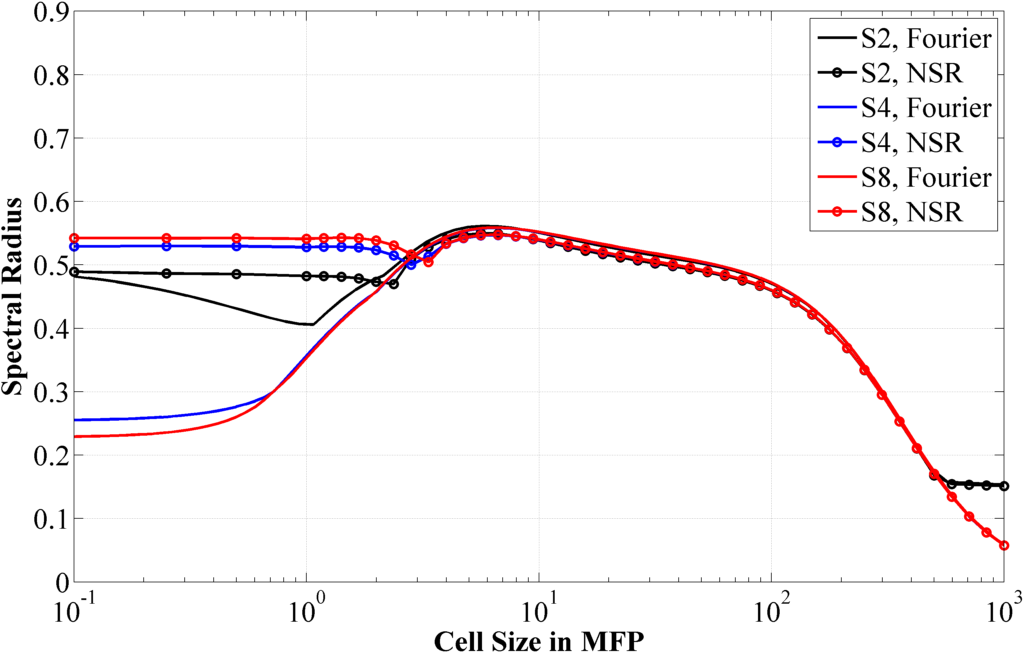
\includegraphics[width=\textwidth]{figures/SI_MIP_hex_C=4_LS2,4,8_F&NSR_PDT.png}
	\end{subfigure}
	\vfill
	\begin{subfigure}[b]{0.48\textwidth}
		\centering
		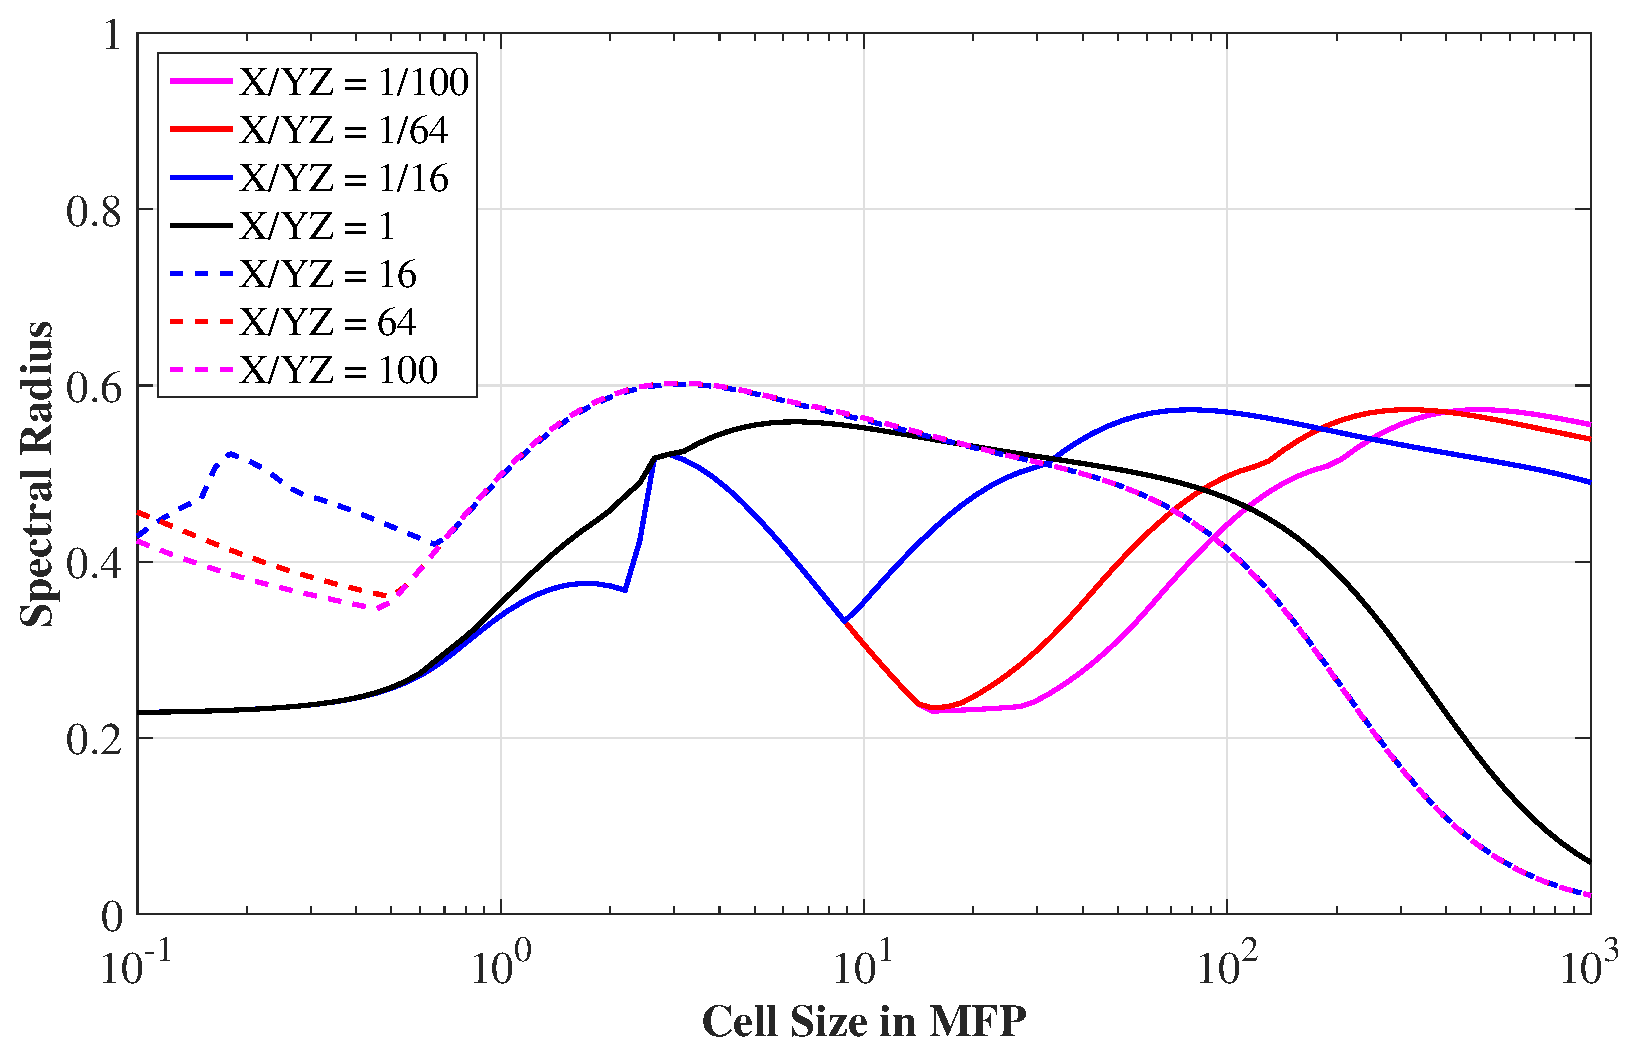
\includegraphics[width=\textwidth]{figures/SI_MIP_hex_LS8_C=1_AR.eps}
	\end{subfigure}
	\hfill
	\begin{subfigure}[b]{0.48\textwidth}
		\centering
		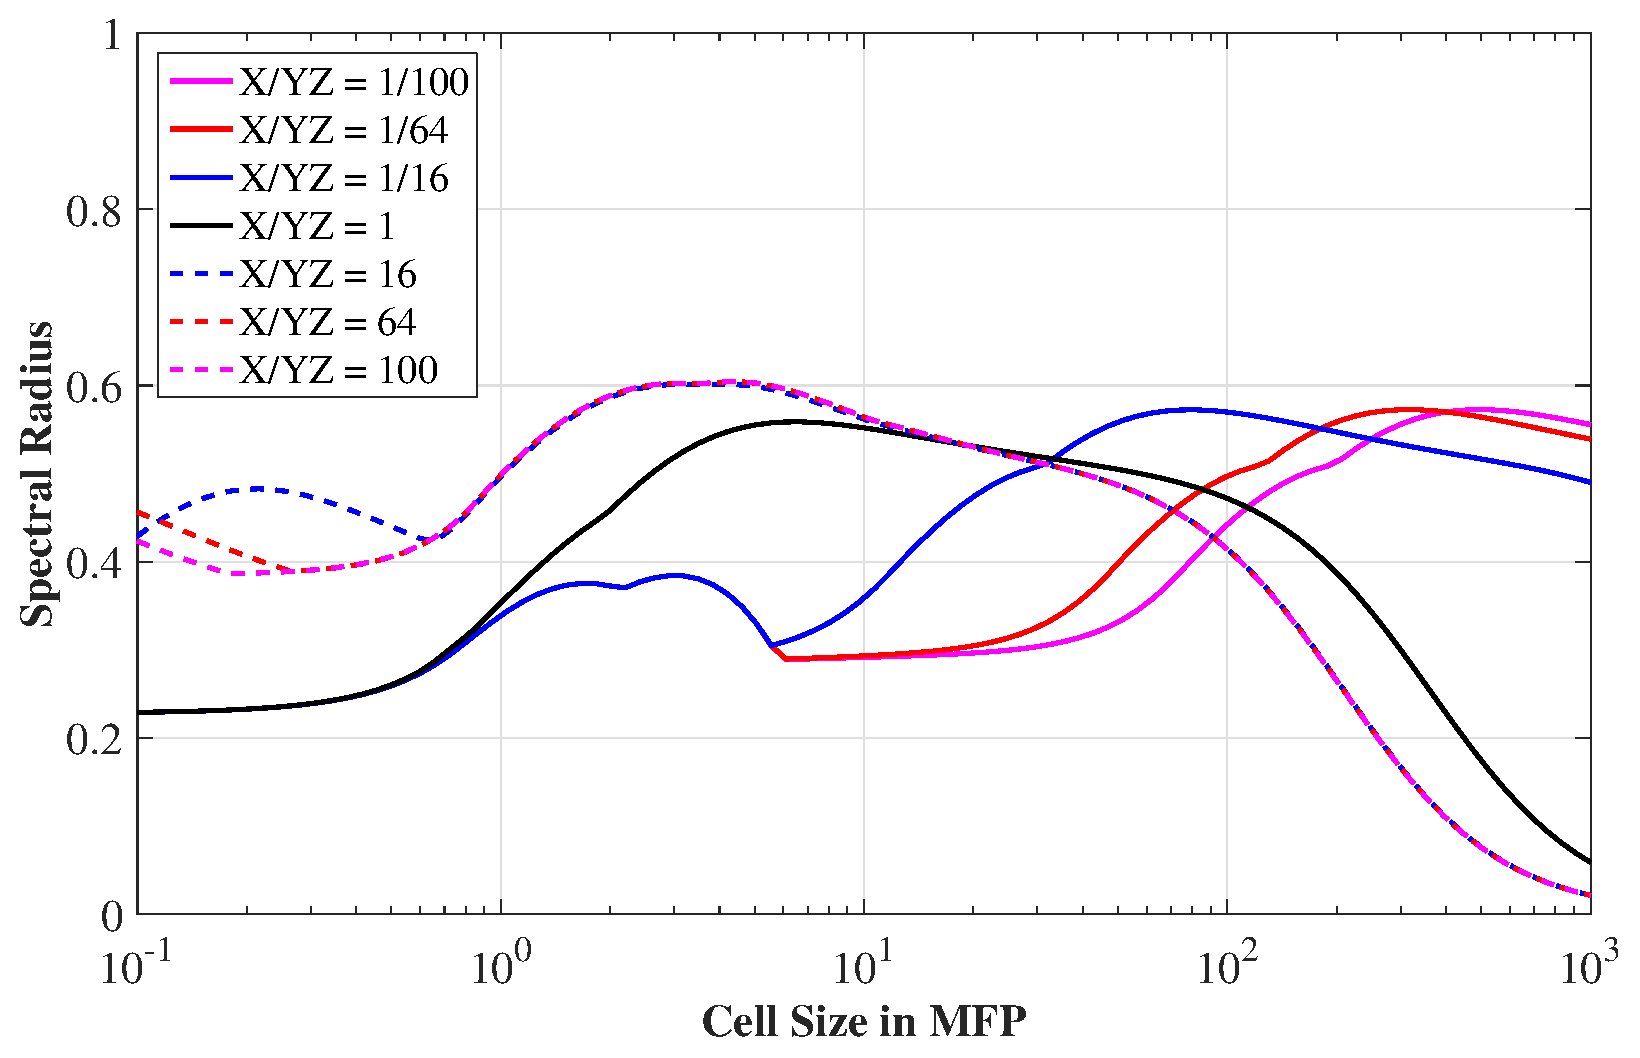
\includegraphics[width=\textwidth]{figures/SI_MIP_hex_LS8_C=4_AR.eps}
	\end{subfigure}
\caption{Fourier and numerical spectral radii results on the unit cube with PWL basis functions and varying $S_N$ order (top). Fourier spectral radii results on parallelipipeds with varying aspect ratios with PWL basis functions and $S_8$ order (bottom). MIP penalty constant: $c=1$ (left) and $c=4$ (right).}
\label{fig::fourier_NSR}
\end{figure}

\begin{figure}
\centering
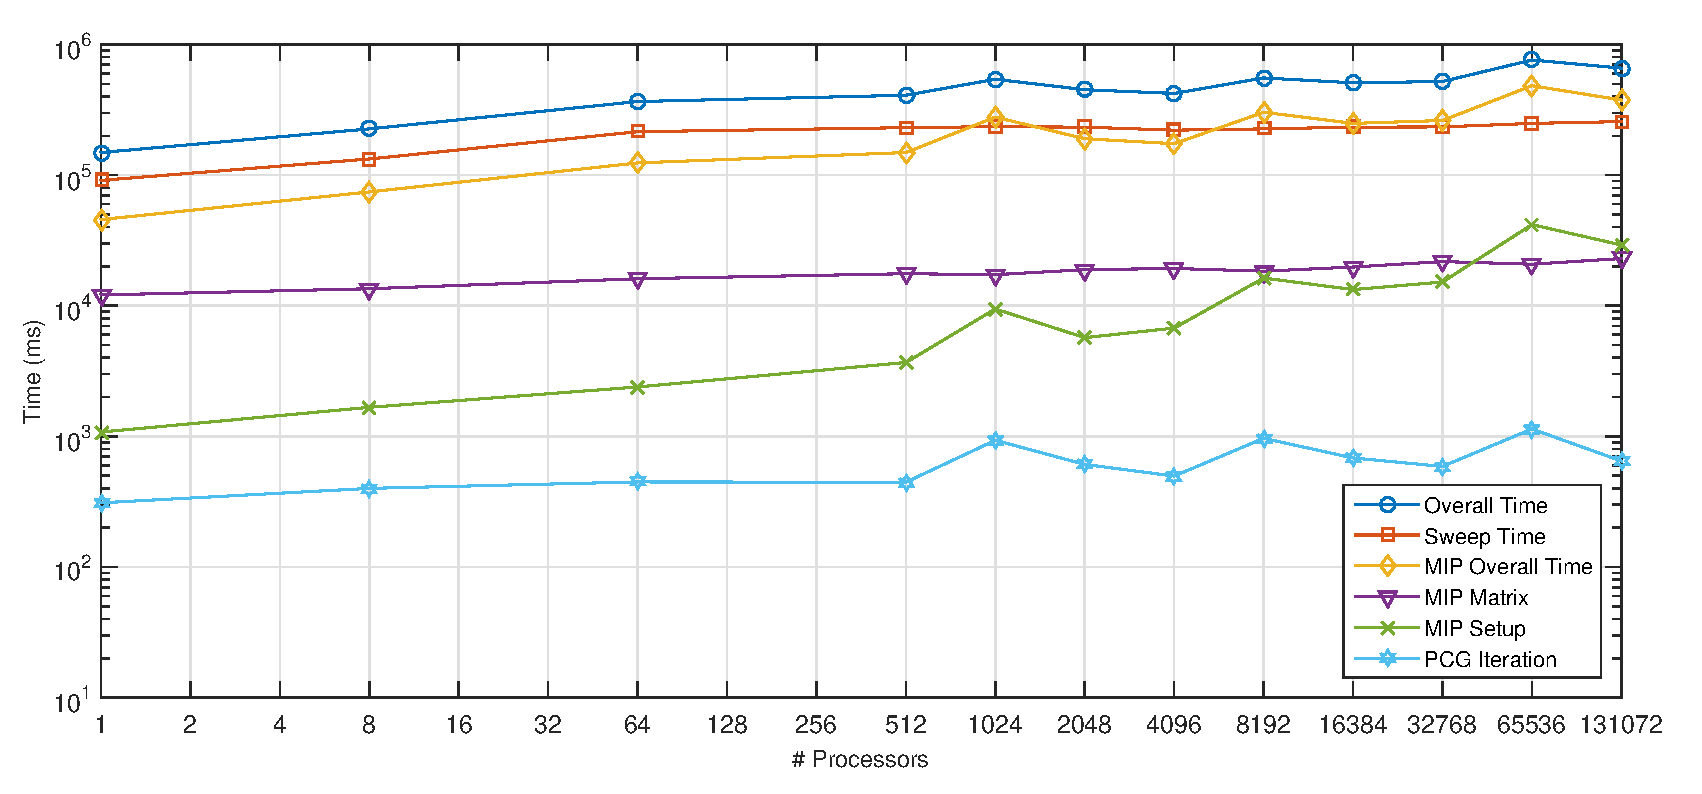
\includegraphics[width=0.90\textwidth]{figures/Vulcan_DSA_Timing.eps}
\caption{Timing data for MIP DSA preconditioning in the PDT code on the VULCAN cluster.}
\label{fig::Vulcan_MIP_Timing}
\end{figure}

%%%%%%%%%%%%%%%%%%%
\subsubsection{Thermal Upscatter Acceleration}
\label{sec::CW_DSA_Upscatter}

For this dissertation work, we will also analyze the benefits and scalability of DSA preconditioning to real-world problems. This can require the ability to efficiently converge the scattering source for a large multigroup problem. However, if there is appreciable up-scattering from the thermal energy groups, then the system can act optically thick which leads to arbitrarily-slow convergence. In particular, systems that are dominated by the thermal scattering off graphite or heavy-water behave in this manner. In this work, we will analyze three different thermal neutron upscattering acceleration techniques. The first method we will analyze is a multigroup richardson acceleration in Section \ref{sec::CW_DSA_Upscatter_Rich}. We will then analyze the Two-Grid acceleration method and a variant in Section \ref{sec::CW_DSA_Upscatter_TG}.

%%%%%%%%%%%%%%%%%%%
\paragraph{Multigroup Richardson Acceleration}
\label{sec::CW_DSA_Upscatter_Rich}

The first thermal neutron upscattering acceleration method we will consider is a multigroup richardson acceleration technique. If we lump all the $G$ thermal groups into a single set and solve simultaneously, then the transport iterations will look like the following:

\begin{equation}
\label{eq::MG_full_eq_it}
{\bf L}_{gg} \Psi_g^{(k+1/2)} =  {\bf M} \sum_{g'=1}^G {\bf S}_{g g'} \Phi_{g'}^{(k)} + {\bf Q}_g.
\end{equation}

\noindent For each thermal transport sweep, we use the scattering source built from the previous sweep and solve for all $G$ thermal groups at once. If we form a new equation by using the exact solution of Eq. (\ref{eq::MG_full_eq_it}) and subtracting Eq. (\ref{eq::MG_full_eq_it}) from this new equation, we get the following error equation, 

\begin{equation}
\label{eq::MG_full_eq_err}
{\bf L}_{gg} \delta \Psi_g^{(k+1/2)} - {\bf M} \sum_{g'=1}^G {\bf S}_{g g'} \delta \Phi_{g'}^{(k+1/2)}=  {\bf M} \sum_{g'=1}^G {\bf S}_{g g'}\left( \Phi_{g'}^{(k+1/2)}- \Phi_{g'}^{(k)} \right)
\end{equation}

\noindent where the notation for the iteration error in Eq. (\ref{eq::CW_delta_fluxes}) has been extended to group-wise errors. For this acceleration method, we do not solve a multigroup diffusion equation. Instead we form our low-order DSA operator by taking the 0th and 1st order moments of Eq. (\ref{eq::MG_full_eq_err}) and perform an energy collapse to form the 1-group, averaged diffusion equation,

\begin{equation}
\label{eq::EC_diff_eq}
- \vec{\nabla} \cdot \Big< D \Big> \vec{\nabla} \epsilon^{(k+1/2)} +  \Big< \sigma \Big> \epsilon^{(k+1/2)} = \Big< R \Big> ,
\end{equation}

\noindent where the multigroup error has been factorized: $\delta \Phi_g^{(k+1/2)} (\vec{r}) = \xi_g \epsilon (\vec{r})$. The error is split into a space-dependent modulation funciton, $\epsilon (\vec{r})$, and a group-wise spectral shape function, $\xi_g$. For each material present in the problem, the spectral shape function is determined by calculating the eigenvector corresponding to the largest eigenvalue of the following,

\begin{equation}
\label{eq::rich_accel_EC}
{\bf T} ^{-1} {\bf S}_0 \xi = \rho \xi ,
\end{equation}

\noindent where

\begin{equation}
\label{eq::rich_accel_EC_sum}
\sum_{g=1}^G \xi_g = 1 .
\end{equation}

\noindent Using the calculated spectral functions of Eq. (\ref{eq::rich_accel_EC}), the remaining energy-collapsed terms of Eq. (\ref{eq::EC_diff_eq}) can be computed in the following manner,

\begin{equation}
\label{eq::EC_diff_terms}
\begin{aligned}
\Big< D \Big> &= \sum_{g=1}^G D_g \xi_g ,\\
\Big< \sigma \Big> &=  \sum_{g=1}^G \left(   \sigma_{t,g} \xi_g -  \sum_{g'=1}^G \sigma_{s,0}^{g,g'} \xi_{g'} \right)  ,\\
\Big< R \Big> &= \sum_{g=1}^G R_g^{(k+1/2)},
\end{aligned} 
\end{equation}

\noindent where the group-wise residual terms are formed from the 0th moments of the scattering matrix:

\begin{equation}
\label{eq::rich_residual}
R_g^{(k+1/2)} =  \sum_{g'=1}^G {\bf S}_{g, g',0} \left(  \Phi_{g',0}^{(k+1/2)} - \Phi_{g',0}^{(k)}  \right).
\end{equation}

\noindent Finally, once the space-dependent modulation function is calculated for a half-iterate, $\epsilon^{(k+1/2)}$, then the update of the transport solution is simply:

\begin{equation}
\label{eq::rich_update}
\Phi_g^{(k+1)} =  \Phi_g^{(k+1/2)} + \xi_g  \epsilon^{(k+1/2)}.
\end{equation}

%%%%%%%%%%%%%%%%%%%
\paragraph{Two-Grid Acceleration and a Variant}
\label{sec::CW_DSA_Upscatter_TG}

The second thermal neutron upscattering acceleration method we will analyze is the Two-Grid (TG) acceleration technique \cite{adams1993two}. The TG method has some similarities to the multigroup richardson acceleration of Section \ref{sec::CW_DSA_Upscatter_Rich}, but some key differences as well. First, instead of solving all $G$ thermal groups simultaneously in a transport sweep, we employ a Gauss-Seidel procedure in energy. This means that we march through the thermal groups in an outer iteration 1 at a time and converge the inner iterations as we go. This leads to a different set of transport iterations:

\begin{equation}
\label{eq::GS_it}
{\bf L}_{gg} \Psi_g^{(k+1/2)} = {\bf M} \sum_{g'=1}^g {\bf S}_{g g'} \Phi_{g'}^{(k+1/2)} + {\bf M} \sum_{g'=g+1}^G {\bf S}_{g g'} \Phi_{g'}^{(k)} + {\bf Q}_g .
\end{equation}

We can then form an equation for the iteration error,

\begin{equation}
\label{eq::TG_full_eq_err}
{\bf L}_{gg} \delta \Psi_g^{(k+1/2)} - {\bf M} \sum_{g'=1}^G {\bf S}_{g g'} \delta \Phi_{g'}^{(k+1/2)}=  {\bf M} \sum_{g'=g+1}^G {\bf S}_{g g'}\left( \Phi_{g'}^{(k+1/2)}- \Phi_{g'}^{(k)} \right) ,
\end{equation}

\noindent where we can obviously see that the residual error is only the upscatter portion of the scattering matrix. The only other differences lie in how we perform our interpolation and projection in energy space. We use the same 1-group energy collapsed diffusion equation and terms from Eqs. (\ref{eq::EC_diff_eq}) and (\ref{eq::EC_diff_terms}), respectively. We simply change how the spectral shape and residuals are calculated. If we decompose the 0th order scattering matrix into its strictly-lower, ${\bf S}_{L,0}$, strictly-upper, ${\bf S}_{U,0}$, and strictly-diagonal portions, ${\bf S}_{D,0}$, then the spectral shape can be computed from,

\begin{equation}
\label{eq::TG_accel_EC}
\left( {\bf T}- {\bf S}_{L,0} - {\bf S}_{D,0} \right)^{-1}  {\bf S}_{U,0}  \xi = \rho \xi,
\end{equation}

\noindent and the diffusion equation residual from,

\begin{equation}
\label{eq::TG_residual}
R_g^{(k+1/2)} =  \sum_{g'=g+1}^G {\bf S}_{g, g',0} \left(  \Phi_{g',0}^{(k+1/2)} - \Phi_{g',0}^{(k)}  \right).
\end{equation}

\noindent Then, following an outer iteration where we have converged the inners in each group, we update the transport iterations with the same correction as Eq. (\ref{eq::rich_update}).

The final neutron upscattering acceleration method that we will investigate is a slightly modified form of TG. In the appendix of their paper, Evans, Clarno, and Morel propsed a Modified Transport Two-Grid (MTTG) acceleration scheme for use with transport synthetic acceleration \cite{evans2010transport}. We will utilize their same methodology but use the diffusion equation as our low-order operator instead of angularly-coarse transport equation to form the Modified Two-Grid (MTG) scheme. It is almost identical to the TG scheme, but we simply do not converge the inner iterations of the Gauss-Seidel process (in fact we only need to employ 1 transport sweep per energy group). The transport iterations then have a slightly modified structure,

\begin{equation}
\label{eq::MTG_it}
{\bf L}_{gg} \Psi_g^{(k+1/2)} = {\bf M} \sum_{g'=1}^{g-1} {\bf S}_{g g'} \Phi_{g'}^{(k+1/2)} + {\bf M} \sum_{g'=g}^G {\bf S}_{g g'} \Phi_{g'}^{(k)} + {\bf Q}_g .
\end{equation}

Then, after 1 outer iteration through all the thermal groups (only 1 sweep per group), we apply the correction from Eq. (\ref{eq::rich_update}). The only difference is that the spectral shape is calculated from the modified equation, $\left( {\bf T}- {\bf S}_{L,0} \right)^{-1} \left( {\bf S}_{D,0}+ {\bf S}_{U,0} \right) \xi = \rho \xi $, and the residual for the diffusion solve becomes,

\begin{equation}
\label{eq::MTG_residual}
R_g^{(k+1/2)} =  \sum_{g'=g}^G {\bf S}_{g, g',0} \left(  \Phi_{g',0}^{(k+1/2)} - \Phi_{g',0}^{(k)}  \right).
\end{equation}

%%%%%%%%%%%%%%%%%%%
\paragraph{The IM1 Experiment}
\label{sec::CW_DSA_Upscatter_IM1}

We seek to test our thermal upscattering acceleration methods on a real-world physical problem. We have chosen to test these methods on the IM1 experiment which is seeking to determine an effective impurity model for the contamination present within graphite bricks. The problem consists of multiple materials and significantly heterogeneous configuration as seen in Figure \ref{fig::IM1_layouts_a}. The materials consist of air, wood, Boral, high-density polyethylene (HDPE), borated HDPE (B-HDPE), an AmBe source, graphite, steel supports, aluminum supports, and a BF3 detector. The simulations are run with 99 energy groups and with a PGLC quadrature set consisting of 30 polar and 6 azimuthal angles in each octant.

\begin{figure}
\centering
	\begin{subfigure}[b]{0.375\textwidth}
		\centering
		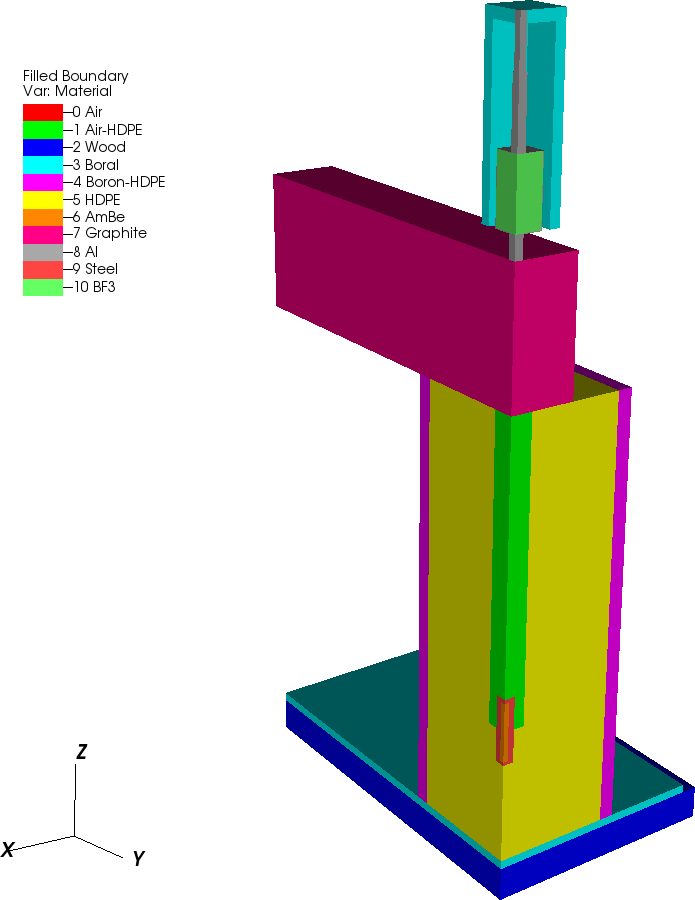
\includegraphics[width=\textwidth]{figures/IM1_configuration_Rev1.png}
		\caption{}
		\label{fig::IM1_layouts_a}
	\end{subfigure}
	\hfill
	\begin{subfigure}[b]{0.375\textwidth}
		\centering
		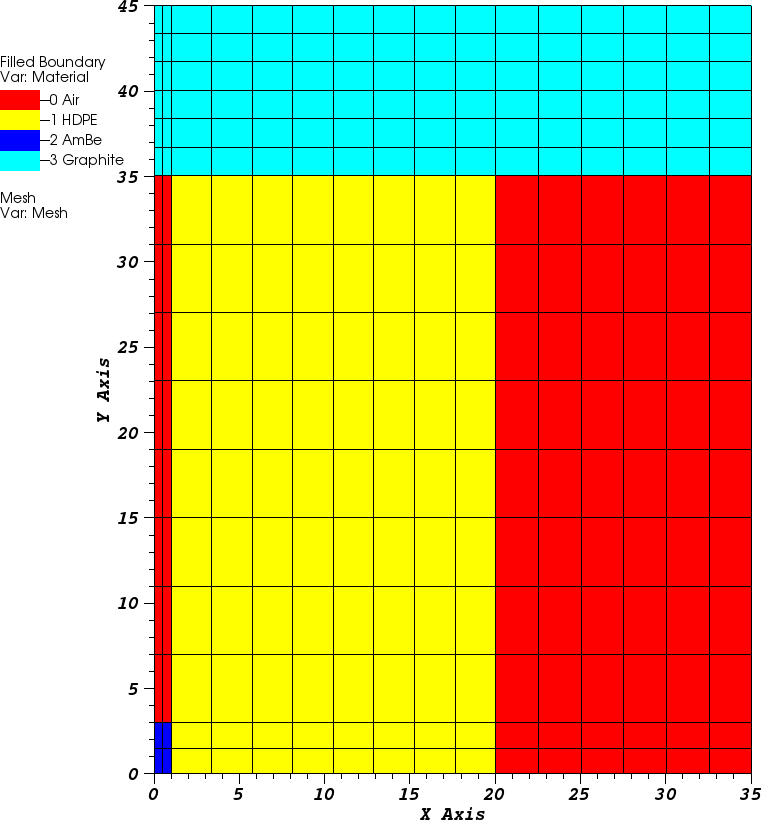
\includegraphics[width=\textwidth]{figures/2D_IM1_Variant_Layout.png}
		\caption{}
		\label{fig::IM1_layouts_b}
	\end{subfigure}
\caption{IM1 problem layout (left) and a simplified 2D variant (right).}
\label{fig::IM1_layouts}
\end{figure} 

Because the full 3D IM1 simulation setup is large, we wished to first perform some simplified analysis of the acceleration methods on a smaller problem configuration. Figure \ref{fig::IM1_layouts_b} shows a simple 2D analogue of the IM1 problem with a reflecting boundary on the left face and the only materials being AmBe, air, graphite and HPDE. We have performed theoretical analysis of the different acceleration methods on the various materials present in the IM1 experiment. Table \ref{tab::IM1_inf_med_SR} gives the infinite medium spectral radius for all the IM1 materials for both the unaccelerated and accelerated upscatter methods. In this case, the unaccelerated results simply perform the transport iterations of Eqs. (\ref{eq::MG_full_eq_it}), (\ref{eq::GS_it}), and (\ref{eq::MTG_it}) without their corresponding acceleration steps. From the table, we can clearly see that TG acceleration provides the best convergence properties for all the IM1 materials. However, that does not necessarily mean that TG will give us the best overall performance when it comes to simulation run time.


\begin{table}
\caption{Infinite medium spectral radii of the IM1 materials for the three thermal neutron upscattering methods. We include both the unaccelerated (U) and accelerated (A) cases.}
\centering
\def\arraystretch{1.2}
\begin{tabular}{|c||c|c||c|c||c|c|}
\hline
Material & U. Rich. & A. Rich. & U. TG & A. TG & U. MTG & A. MTG \\ \hline
Graphite & 0.9993 & 0.9613 & 0.9883 &0.4084 & 0.9993 & 0.9604 \\
HDPE & 0.9943 & 0.8015 & 0.8916 & 0.4343&  0.9918 & 0.7527 \\
B-HDPE &0.1336 & 0.1223  & 0.0258 & 0.0177 &  0.1331 & 0.1221 \\
Wood & 0.9915 & 0.5326  & 0.9820 & 0.2101 &  0.9840 & 0.3836 \\
AmBe  & 0.7068 & 0.5596 & 0.4835& 0.2724 & 0.5646 & 0.5554 \\
Steel  & 0.9255 & 0.9215 & 0.6989 & 0.5809 &   0.9243 & 0.9215\\
Boral  & 0.0782 & 0.0602 & 0.0023 & 0.0016 & 0.0782 & 0.0602 \\
BF3   & 0.0351 & 0.0266 & 0.0008& 0.0006 & 0.0351 & 0.0266 \\
Air   & 0.8845 & 0.7896 & 0.7580& 0.5282 &  0.8121 & 0.7828 \\
\hline
\end{tabular}
\label{tab::IM1_inf_med_SR}
\end{table}



%%%%%%%%%%%%%%%%%%%%%%%%%%%%%%%%%%%%%%%%%%%%%%%%%%%%%%%%%%%%%%%%%%%%%%
%%%%%%%%%%%%%%%%%%%%%%%%%%%%%%%%%%%%%%%%%%%%%%%%%%%%%%%%%%%%%%%%%%%%%%
\section{Ongoing Work}
\label{sec::OW}

Thus far, we have presented the overall objectives of the dissertation work and the work that has been completed to this point. There are still several areas of work that need to be completed. They are confined to two distinct areas: 1) remaining theoretical implementation and analysis of the polygonal finite element basis functions and their extension to the quadratic serendipity space and 2) performance analysis of thermal neutron upscattering with  MIP DSA in PDT.

For the analysis of the polygonal basis functions, there are a couple of items left to investigate. First, we need to analyze the convergence rates of the transport equation in a purely-absorbing medium with and without mesh alignment. If the mesh is aligned with the solution discontinuity, then the convergence rates of Eqs. (\ref{eq::bf_conv_rate_h}) and (\ref{eq::bf_conv_rate_DOF}) should be captured. However, if the mesh is not aligned with the analytical discontinuities, then the resulting numerical solutions will only live in either the $H^{1/2}$ or $H^{3/2}$ Sobolev spaces, due to the irregularity of the transport solutions. The final polygonal basis function analysis to perform is to confirm that the quadratic basis functions can exactly capture solutions that are in $\text{span}\left\{  1,x,y,xy,x^2,y^2  \right\}$.

For the DSA work in PDT, there are three items left to investigate. First, we need to complete the last of the numerical experiments to verify the theoretical results of the DSA fourier analysis. This is mostly restricted to the numerical verification of the PHI problem. Second, we will finish our analysis of the effects of partitioning and aggregation on the HYPRE setup and solve times. The raw data for this step has already been collected; it just needs to be properly analyzed and tabulated. Finally, we need to conclude the remaining numerical experiments for the IM1 problem.

%%%%%%%%%%%%%%%%%%%%%%%%%%%%%%%%%%%%%%%%%%%%%%%%%%%%%%%%%%%%%%%%%%%%%%
%%%%%%%%%%%%%%%%%%%%%%%%%%%%%%%%%%%%%%%%%%%%%%%%%%%%%%%%%%%%%%%%%%%%%%
\section{Expected Results and Summary}
\label{sec::ER}

We have presented the dissertation work that has been completed to date as well as the outline for all remaining work. We now quickly summarize the main topical areas of the dissertation project:

\begin{enumerate}
	\item Analyze the 2D linear polygonal basis functions for use in DGFEM transport calculations
	\item Perform the same analysis with the quadratic serendipity basis functions
	\item Perform analysis on benchmark cases using polygonal meshes (including AMR)
	\item Analyze the 2D polygonal basis functions with DSA preconditioning through Fourier/numerical analysis
	\item Analyze the effects of AMR with polygonal basis functions on the MIP DSA PCG iteration counts (with and without bootstrapping)
	\item Extend the analysis of MIP DSA to arbitrary convex 3D polyhedra
	\item Implement MIP DSA in PDT using HYPRE
	\begin{itemize}
		\item Analyze the scalability of the method to high processor counts.
		\item Perform parametric studies on aggregation/partitioning factors to generate a performance model.
		\item Implement and perform analysis of richardson and two-grid acceleration at scale for thermal neutron upscattering problems.
		\item Conclude with real-world numerical experiments on high-fidelity meshes (CERT IM1 problem).
	\end{itemize}
\end{enumerate}

%%%%%%%%%%%%%%%%%%%%%%%%%%%%%%%%%%%%%%%%%%%%%%%%%%%%%%%%%%%%%%%%%%%%%%
%%%%%%%%%%%%%%%%%%%%%%%%%%%%%%%%%%%%%%%%%%%%%%%%%%%%%%%%%%%%%%%%%%%%%%
% References
\bibliographystyle{ans}
\bibliography{references}

\end{document}


